%!TEX root = ../thesis.tex

\chapter{闪电二氧化氮的反演算法} \label{sec:retrieval}

由于地表人为排放的NO$_{\ch{x}}$需经过传输过程才能抵达自由对流层,进而影响该层O$_{\ch{3}}$浓度,
而闪电直接在对流层中上层产生NO并迅速转化为NO$_{\ch{2}}$,
该层的低温导致LNO$_{\ch{2}}$寿命更长,
所以LNO$_{\ch{2}}$可对该层的O$_{\ch{3}}$浓度产生更大的影响。
然而,尽管前人针对LNO$_{\ch{2}}$开展了一系列研究(见\ref{sec:intro_lnox}节),
由于难以原位观测或实验室重现,所以LNO$_{\ch{2}}$的产率仍有很高的不确定性。
本章旨在通过使用卫星观测和云分辨化学模式来改进对LNO$_{\ch{2}}$的估算。

本章余下部分按以下方式组织:
\ref{sec:retrieval_method}节将OMI/TROPOMI观测资料与WRF-Chem模式相结合,
开发了LNO$_2$柱浓度的反演算法,并讨论其适用条件及范围;
\ref{sec:retrieval_comp}节将该算法应用于北美大陆地区,并将所得的LNO$_2$产率与前人研究进行对比,分析其差异性和不确定性;
最后是本章小结。

\section{基于卫星遥感的闪电二氧化氮反演} \label{sec:retrieval_method}

\subsection{算法基础} \label{sec:amf_definition}

为了得到对流层LNO$_{\ch{2}}$或LNO$_{\ch{x}}$的垂直柱浓度,本研究基于$AMF_{\ch{trop}}$将分母改成LNO$_{\ch{2}}$或LNO$_{\ch{x}}$的垂直积分:
\begin{equation} \label{eq:AMF_LNO2}
AMF_{\ch{LNO_2}} = \frac{(1-f_r) \int_{p_{surf}}^{p_{tp}} w_{clear}(p) NO_2(p) \: dp + f_r \int_{p_{cloud}}^{p_{tp}} w_{cloudy}(p) NO_2(p) \: dp}{\int_{p_{surf}}^{p_{tp}} LNO_2(p) \: dp}
\end{equation}

当研究区域为清洁区域,式(\ref{eq:AMF_LNO2})的分子可用LNO$_{\ch{2}}$代替NO$_{\ch{2}}$,即
\begin{equation} \label{eq:AMF_LNO2clean}
AMF_{\ch{LNO_2Clean}} = \frac{(1-f_r) \int_{p_{surf}}^{p_{tp}} w_{clear}(p) LNO_2(p) \: dp + f_r \int_{p_{cloud}}^{p_{tp}} w_{cloudy}(p) LNO_2(p) \: dp}{\int_{p_{surf}}^{p_{tp}} LNO_2(p) \: dp}
\end{equation}

为了与前人对比,本研究定义了其他两种云上的AMF,
\begin{equation} \label{eq:AMF_NO2Vis}
AMF_{\ch{NO_2Vis}} = \frac{(1-f_r) \int_{p_{surf}}^{p_{tp}} w_{clear}(p) NO_2(p) \: dp + f_r \int_{p_{cloud}}^{p_{tp}} w_{cloudy}(p) NO_2(p) \: dp}{(1-f_g) \int_{p_{surf}}^{p_{tp}} NO_2(p) \: dp + f_g \int_{p_{cloud}}^{p_{tp}} NO_2(p) \: dp}
\end{equation}
\begin{equation} \label{eq:AMF_LNO2Vis}
AMF_{\ch{LNO_2Vis}} = \frac{(1-f_r) \int_{p_{surf}}^{p_{tp}} w_{clear}(p) NO_2(p) \: dp + f_r \int_{p_{cloud}}^{p_{tp}} w_{cloudy}(p) NO_2(p) \: dp}{(1-f_g) \int_{p_{surf}}^{p_{tp}} LNO_2(p) \: dp + f_g \int_{p_{cloud}}^{p_{tp}} LNO_2(p) \: dp}
\end{equation}
其中$f_g$为云几何分数,各式中的NO$_{\ch{2}}$和LNO$_{\ch{2}}$廓线均来自于WRF-Chem的模拟结果。
由于污染地区LNO$_{\ch{2}}$柱浓度的估算
需要同时考虑详细的LNO$_{\ch{2}}$和人为污染NO$_{\ch{2}}$的分布,
因此本研究使用WRF-Chem高分辨率模拟结果来获得AMF,进而计算LNO$_{\ch{2}}$的柱浓度。
在美国大陆的模拟研究中使用的WRF-Chem版本为3.5.1,水平网格大小为12 km $\times$ 12 km (图\ref{fig:us_domain}a),垂直层数为29层,时间步长为72 s。
气象条件的初始场和边界场为时间分辨率3小时的北美区域再分析(NARR)数据集,
每3小时应用一次边界条件和四维数据分析(FDDA)逼近,
其中温度、水汽和水平风以0.0003 s$^{-1}$ 的系数逼近\citep{Laughner.2017}。
微物理过程采用Lin方案\citep{Lin.1983},积云参数化为Grell 3D方案\citep{Grell.1993a,Grell.2002a},
长波辐射采用RRTM方案\citep{Iacono.2008},短波辐射采用Goddard方案,
陆面过程使用Noah陆面模式\citep{Koren.1999},边界层采用YSU方案\citep{Hong.2006}。
闪电参数化采用基于对流参数化的中性浮力水平\citep{Pickering.1992},云闪与地闪的比例基于\citet{Boccippio.2001}.

\begin{figure}[H]
\centering
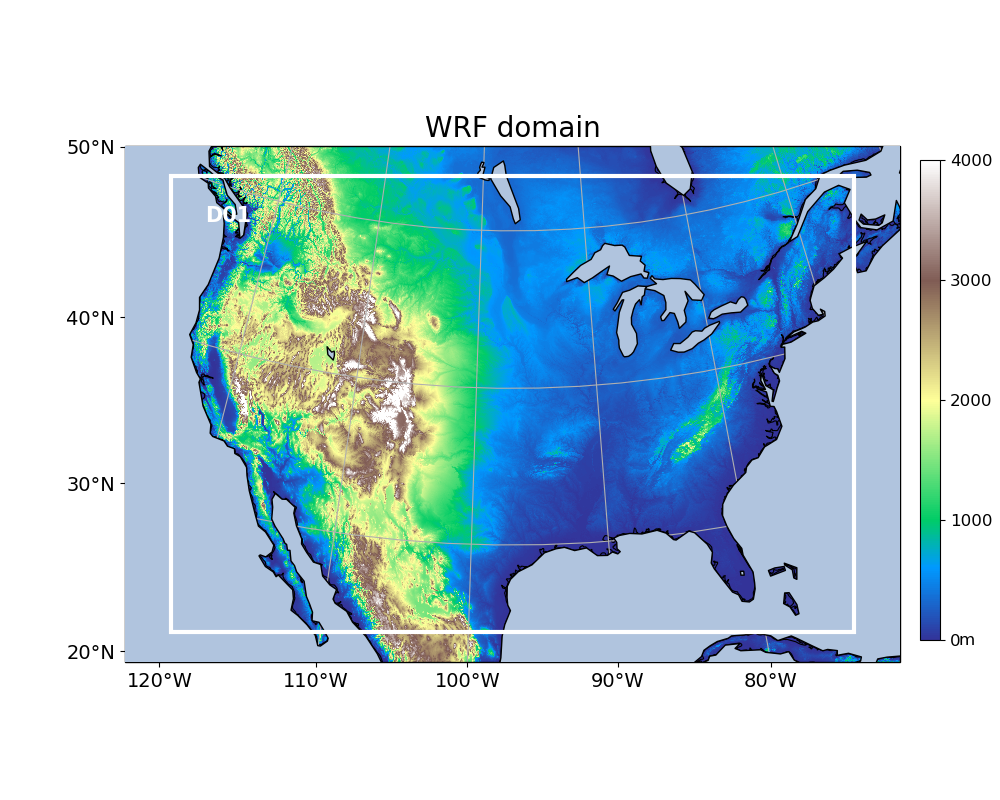
\includegraphics[width=0.85\textwidth]{./figures/us_domain.png}
\caption{WRF-Chem 模拟区域和地形高度(m),网格数为 350 $\times$ 290,水平分辨率为 12 km。 \\
Figure \ref{fig:us_domain}. Domain and terrain height (m) of the WRF-Chem simulation with 350 x 290 grid cells and a horizontal resolution of 12 km.}
\label{fig:us_domain}
\end{figure}

化学的初始场和边界场采用臭氧和相关化学示踪剂模式第4版[MOZART-4,\citet{Emmons.2010}]的输出场。
人为排放由2011年美国国家排放清单(NEI)驱动,并根据环境保护署年度总排放量,按模拟的年份进行调整\citep{EPA.2015}。
生物排放使用MEGAN源,化学机制是区域大气化学机制第2版[RACM2,\citet{Goliff.2013}],
并由\citet{Browne.2014}和\citet{Schwantes.2015}进行了更新。
此外,LNO$_{\ch{x}}$参数化采用每次闪电产生200 mol NO,调整因子为1,以下简称“1$\times$200 mol NO每闪电”。
WRF-Chem中LNO垂直分布采用基于\citet{Ott.2010}的双峰型闪电NO(LNO)廓线\citep{Laughner.2017},
LNO和LNO$_{\ch{2}}$廓线是指开启和关闭LNO排放的模拟之间各自垂直廓线的差异。


\subsection{算法的应用条件}

首先本研究使用恒定值网格化法,将公式(\ref{eq:AMF_LNO2})所得的LNO$_{\ch{2}}$垂直柱浓度(V$_{\ch{LNO_2}}$)分配至0.05$^{\circ}$ $\times$ 0.05$^{\circ}$网格\citep{Kuhlmann.2014}。
接着在 1$^{\circ}$ $\times$ 1$^{\circ}$的网格中进行分析,要求每个网格至少有50个有效的0.05$^{\circ}$ $\times$ 0.05$^{\circ}$网格数据,从而最小化噪点。
具体筛选条件和主要计算步骤如下。

云辐射分数(CRF,CRF $\geq$ 70\%,CRF $\geq$ 90\%,CRF = 100\%)和 云压(CP,CP $\leq$ 650 hPa)
通常是判断OMI像素是否包含深对流云的标准\citep{Ziemke.2009,Choi.2014,Pickering.2016}。
此外本研究将另一个云分数(CF)标准应用于 WRF-Chem 的模拟结果,以确保成功模拟出对流。
具体而言,CF是由 Xu-Randall 方法计算的 350--400 hPa 之间的最大云分数\citep{Xu.1996,Strode.2017}。
本研究根据\citet{Strode.2017}的建议,选择350--400 hPa的CF $\geq$ 40\%来判断模拟所处的网格是多云或晴空,
可避免模拟高云中的偏差。

除了云特性之外,OMI能探测到新生LNO$_{\ch{2}}$的另一条件为一段时间内有足够的闪电或闪击,
其中时间窗口 (t$_{window}$) 是 OMI 过境之前的时间段。
\citet{Lapierre.2020}利用1$^{\circ}$ $\times$ 1$^{\circ}$网格的对角线长度和OMI过境时美国大陆上空500--100 hPa的平均风速计算得到t$_{window}$为2.4 h。
同时,\citet{Lapierre.2020}定义在t$_{window}$时间段内至少发生2400次闪电或8160次闪击的网格,才能提供足够的LNO$_{\ch{2}}$给OMI探测。
\citet{Bucsela.2019}的研究表明,低频率的闪电具有更高的LNO$_{\ch{2}}$产率,而该段数据在\citet{Lapierre.2020}研究中被剔除。
通过比较使用每个网格至少2400次闪电和至少1次闪电的标准所得结果,本研究也得到相同的结论(图\ref{fig:us_flash_threshold})。
由于本论文的研究重点是开发一种新的AMF,并将计算结果与使用类似闪电阈值的其他产品进行比较\citep{Pickering.2016,Lapierre.2020},
因此本研究接下来使用相同的“至少2400次闪电”标准来进行结果分析。


\begin{figure}[H]
\centering
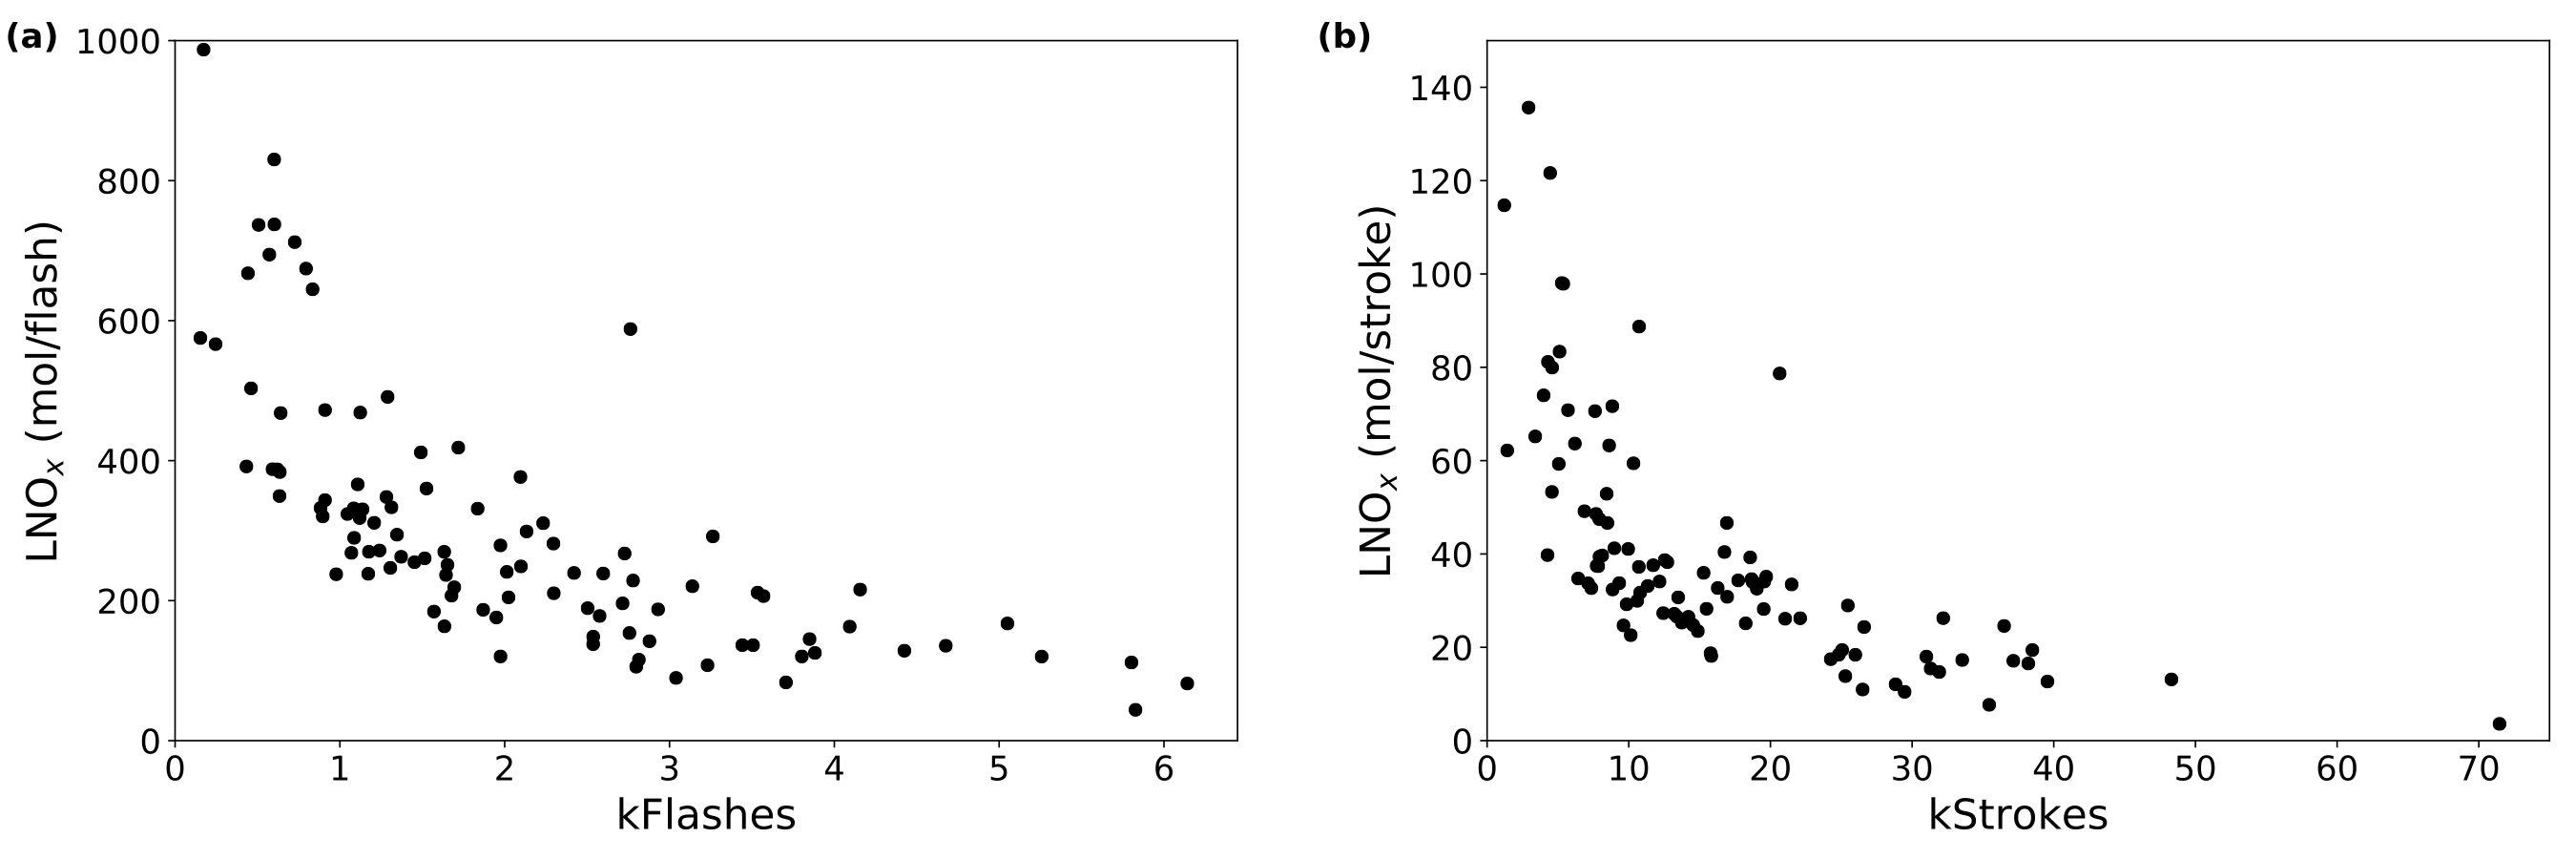
\includegraphics[width=0.9\textwidth]{./figures/us_flash_threshold.png}
\caption{
(a) 每日 LNO$_{\ch{x}}$ 产率与 ENTLN 总闪的关系,筛选条件为CRF $\geq$ 90\% 且1$^{\circ}$ $\times$ 1$^{\circ}$网格中至少有1次闪电;
 (b) 与 (a) 相同,但针对闪击。\\
Figure \ref{fig:us_flash_threshold}. (a) Daily LNO$_{\ch{x}}$ production efficiencies versus ENTLN total flashes data, with CRF $\geq$ 90\% and a flash threshold of 1 flash box$^{-1}$.
(b) Same as (a) but for strokes.}
\label{fig:us_flash_threshold}
\end{figure}


为确保WRF-Chem成功模拟出闪电,并考虑到闪电参数化的不确定性,本研究将每个1$^{\circ}$ $\times$ 1$^{\circ}$网格模拟的总闪电(TL)阈值设置为1000,该阈值低于ENTLN闪电观测使用的阈值。
针对除LNO$_{\ch{2}}$之外的其他NO$_{\ch{2}}$源,本研究定义了模拟的云上闪电NO$_{\ch{2}}$柱浓度($V_{\ch{LNO2Vis}}$)
与云上NO$_{\ch{2}}$柱浓度($V_{\ch{NO2Vis}}$)之比,来判断OMI是否可以检测到足够的LNO$_{\ch{2}}$,
若该比值$\geq$50\%,则表明云层上方超过一半的NO$_{\ch{2}}$具有LNO$_{\ch{2}}$源。
此外还需考虑氧化有关的NO$_{\ch{2}}$寿命,
\citet{Nault.2017}的研究表明NO$_{\ch{2}}$在对流附近的寿命($\tau$)为$\sim$3 h,故NO$_{\ch{2}}$的初始值可由式(\ref{eq:inition})求解。

\begin{equation} \label{eq:inition}
LNO_2(0) = LNO_2(\mathrm{OMI})\ e^{0.5t/\tau}
\end{equation}

其中$LNO_2(0)$是在时间 t=0 时刻排放的LNO$_{\ch{2}}$摩尔数,$LNO_2(\mathrm{OMI})$是在 OMI 过境时测得的LNO$_{\ch{2}}$摩尔数,
0.5t是穿过网格的时间即1.2 h(假设闪电出现在每个1$^{\circ}$ $\times$ 1$^{\circ}$网格的中心)。
每个网格中的LNO$_{\ch{2}}$摩尔数为其中所有0.05$^{\circ}$ $\times$ 0.05$^{\circ}$像素的V$_{\ch{LNO_2}}$平均值与网格面积的乘积。
最后,有两种方法可用于估算季节性平均LNO$_{\ch{2}}$每闪电、LNO$_{\ch{x}}$每闪电、LNO$_{\ch{2}}$每闪击和 LNO$_{\ch{x}}$每闪击:

(1)求和法,将LNO$_{\ch{2}}$或LNO$_{\ch{x}}$的总和除以5--8月中每个1$^{\circ}$ $\times$ 1$^{\circ}$网格里发生的闪电或闪击总数;

(2)线性回归方法,将线性回归应用于LNO$_{\ch{2}}$或LNO$_{\ch{x}}$和闪电或闪击的日均值。

% \subsection{适合反演闪电氮氧化物的条件} \label{subsec:criteria}

根据以上条件,本研究定义了六种不同的筛选条件组合(表\ref{table:Abbreviations}),并将线性回归法应用于原始数据。


\begin{table}[H]
\caption{本研究中各标准的缩写定义\\Table \ref{table:Abbreviations}. Definitions of the abbreviations for the criteria used in this study.}
\scriptsize
\begin{tabular}{ll}
\thickline
缩写$^a$ & 全称 [来源] \\
\thickline
CRF                             & 云辐射分数 Cloud radiance fraction [OMI] \\
CP                              & 云压Cloud pressure [OMI] \\
CF                              & 云分数 Cloud fraction [WRF-Chem] \\
TL                              & 总闪电数 Total lightning [WRF-Chem] \\
ratio                           & $V_{\ch{LNO2Vis}}$ / $V_{\ch{NO2Vis}}$ [WRF-Chem] \\
CRF$\alpha$\_ENTLN                   & CRF $\geq$ $\alpha$ + ENTLN 闪电(闪击)$\geq$ 2400(8160)[ENTLN]\\
CRF$\alpha$\_CF40\_ENTLN              & CRF $\geq$ $\alpha$ + ENTLN 闪电(闪击)$\geq$ 2400(8160)+ CF $\geq$ 40\% \\
CRF$\alpha$\_ENTLN\_TL1000            & CRF $\geq$ $\alpha$ + ENTLN 闪电(闪击)$\geq$ 2400(8160)+ TL $\geq$ 1000 \\
CRF$\alpha$\_CF40\_ENTLN\_TL1000      & CRF $\geq$ $\alpha$ + ENTLN 闪电(闪击)$\geq$ 2400(8160)+ CF $\geq$ 40\% + TL $\geq$ 1000 \\
CRF$\alpha$\_ENTLN\_TL1000\_ratio50   & CRF $\geq$ $\alpha$ + ENTLN 闪电(闪击)$\geq$ 2400(8160)+ TL $\geq$ 1000 + ratio $\geq$ 50\% \\
CRF$\alpha$\_CF40\_ENTLN\_TL1000\_ratio50 & CRF $\geq$ $\alpha$ + ENTLN 闪电(闪击)$\geq$ 2400(8160)+ CF $\geq$ 40\% + TL $\geq$ 1000 + ratio $\geq$ 50\% \\
CRF$\alpha$\_ENTLN1(3.4)\_TL1\_ratio50    & CRF $\geq$ $\alpha$ + ENTLN 闪电(闪击)$\geq$ 1(3.4)+ TL $\geq$ 1 + ratio $\geq$ 50\% \\
\thickline
\end{tabular}
\begin{tablenotes}
\linespread{1}\footnotesize
\item $^a$ $\alpha$有三种选择:70\%、90\%以及100\%。
\item $^a$ $\alpha$ has three options: 70\%, 90\% and 100\%.
\end{tablenotes}
\label{table:Abbreviations}
\end{table}


\begin{table}[H]
\caption{根据表\ref{table:Abbreviations}中的定义得到的LNO$_{\ch{x}}$产率\\Table \ref{table:conditions} LNO$_{\ch{x}}$ production efficiencies for different combinations of criteria defined in Table \ref{table:Abbreviations}.}
\scriptsize
\begin{tabular}{lccccc}
\thickline
条件$^a$ & ENTLN类型$^b$ & LNO$_{\ch{x}}$每闪电 or LNO$_{\ch{x}}$每闪击 & R值 & 截距 (10$^{6}$mol) & 天数$^c$ \\
\thickline
CRF90\_ENTLN                        & 闪电  & 52.1 $\pm$ 51.1 & 0.20 & 0.21  & 99 \\
CRF90\_CF40\_ENTLN                  & 闪电  & 84.2 $\pm$ 31.5 & 0.54 & -0.04 & 70 \\
CRF90\_ENTLN\_TL1000                & 闪电  & 61.9 $\pm$ 49.1 & 0.27 & 0.33  & 83 \\
CRF90\_CF40\_ENTLN\_TL1000          & 闪电  & 63.4 $\pm$ 52.9 & 0.38 & 0.26  & 38 \\
CRF90\_ENTLN\_TL1000\_ratio50       & 闪电  & 54.5 $\pm$ 48.1 & 0.25 & 0.39  & 81 \\
CRF90\_CF40\_ENTLN\_TL1000\_ratio50 & 闪电  & 90.0 $\pm$ 65.0 & 0.46 & 0.15  & 32 \\
CRF90\_ENTLN                        & 闪击 & 6.7 $\pm$ 4.1 & 0.31 & 0.23  & 102 \\
CRF90\_CF40\_ENTLN                  & 闪击 & 10.3 $\pm$ 3.6 & 0.55 & 0.08 & 79 \\
CRF90\_ENTLN\_TL1000                & 闪击 & 7.5 $\pm$ 5.1 & 0.29 & 0.38  & 94 \\
CRF90\_CF40\_ENTLN\_TL1000          & 闪击 & 8.6 $\pm$ 6.2 & 0.39 & 0.27  & 46 \\
CRF90\_ENTLN\_TL1000\_ratio50       & 闪击 & 7.0 $\pm$ 4.8 & 0.29 & 0.42  & 93 \\
CRF90\_CF40\_ENTLN\_TL1000\_ratio50 & 闪击 & 8.9 $\pm$ 7.0 & 0.39 & 0.31  & 40 \\
\thickline
\label{table:conditions}
\end{tabular}
\begin{tablenotes}
\linespread{1}\footnotesize
\item $^a$ 定义见表\ref{table:Abbreviations}。
\item $^b$ ENTLN阈值为OMI过境前2.4小时内 1$^{\circ}$ $\times$ 1$^{\circ}$网格中闪电至少2400次或闪击至少8160次。
\item $^c$ 2014年5--8月中有效的天数。
\item $^a$ These conditions are defined in Table \ref{table:Abbreviations}.
\item $^b$ The thresholds of ENTLN data are 2400 flashes box$^{-1}$ and 8160 strokes box$^{-1}$ during the period of 2.4 h before OMI overpass time.
\item $^c$ The number of valid days with specific criteria in MJJA 2014.
\end{tablenotes}
\end{table}


在CRF90\_ENTLN条件下,有效闪电(闪击)数据对应共有99(102)天。
以闪电类ENTLN数据为例,在 CRF90\_ENTLN\_TL1000\_ratio50 条件下,有效天数从 99 减少至 81,而LNO$_{\ch{x}}$产率从 52.1 $\pm$ 51.1 mol每闪电增加到 54.5 $\pm$ 48.1 mol每闪电。
该结果与 CRF90\_ENTLN\_TL1000 条件下所得的结果几乎相同。
尽管这表明TL筛选条件已足够严格,但最好包括云上LNO$_{\ch{2}}$占比的筛选条件,以防不同的AMF方法中存在一些例外情况。
由于 CF $\geq$ 40\% 会导致有效数据和产率急剧下降,因此本研究仅仅使用 CRF 对数据进行筛选。
最后,本研究选择至少2400次闪电或至少8160次闪击、TL $\geq$ 1000 和云上LNO$_{\ch{2}}$占比 $\geq$ 50\% 作为阈值,来探索三种不同 CRF 条件(CRF $\geq$ 70\%、CRF $\geq$ 90\% 和 CRF = 100\%)对 LNO$_{\ch{x}}$ 估算产生的影响(表\ref{table:CRFs})。

当CRF 标准从 70\% 增加到 90\% 和 100\%时,针对闪电类型的LNO$_{\ch{x}}$产率 从35.7 $\pm$ 36.8 mol每闪电增加到 54.5 $\pm$ 48.1 mol每闪电,然后再降低到20.8 $\pm$ 37.4 mol每闪电,而针对闪击类型的LNO$_{\ch{x}}$产率从4.1 $\pm$ 3.9 mol每闪击提高到 7.0 $\pm$ 4.8 mol每闪击,然后再次下降到2.6 $\pm$ 4.0 mol每闪击(表\ref{table:CRFs})。
当 CRF 从 90\% 增加到 100\% 时,LNO$_{\ch{x}}$ 产率降低,这是因为闪电密度较高而 LNO$_{\ch{x}}$ 较少。
CRF 从 70\% 增加到 90\% 引起的 LNO$_{\ch{x}}$ 产率增大,该现象与\citet{Pickering.2016}的结果相反。
这是由于本研究的方法中考虑了从边界层传输的 NO$_{\ch{2}}$ 污染的影响。
虽然在 CRF $\geq$ 70\% 的地区经常观察到 LNO$_{\ch{2}}$ 的高值\citep{Pickering.2016},但考虑到人为污染 NO$_{\ch{2}}$ 并与\citet{Pickering.2016}和\citet{Lapierre.2020}的结果进行比较,以下分析将基于 CRF $\geq$ 90\% 标准进行讨论分析。


\begin{table}[H]
\caption{在相同ENTLN阈值、TL $\geq$ 1000 和云上LNO$_{\ch{2}}$占比 $\geq$ 50\%的条件下,不同云辐射分数阈值对应的LNO$_{\ch{x}}$产率 \\
Table \ref{table:CRFs}. LNO$_{\ch{x}}$ production efficiencies for different thresholds of CRF with coincident ENTLN data, TL $\geq$ 1000 and ratio $\geq$ 50\%.}
\footnotesize
\begin{tabular}{cccccc}
\thickline
云辐射分数 (\%) & ENTLN类型$^a$    & LNO$_{\ch{x}}$每闪电或LNO$_{\ch{x}}$每闪击
& R值    & 截距 (10$^{5}$mol)  & 天数$^b$ \\
\thickline
70  & 闪电  & 35.7  $\pm$ 36.8 & 0.21 & 4.91 & 85 \\
90  & 闪电  & 54.5  $\pm$ 48.1 & 0.25 & 3.90 & 81 \\
100 & 闪电  & 20.8  $\pm$ 37.4 & 0.13 & 5.67 & 71 \\
70  & 闪击 & 4.1   $\pm$ 3.9  & 0.21 & 5.16 & 96 \\
90  & 闪击 & 7.0   $\pm$ 4.8  & 0.29 & 4.16 & 93 \\
100 & 闪击 & 2.6   $\pm$ 4.0  & 0.14 & 5.41 & 82 \\
\thickline
\end{tabular}
\begin{tablenotes}
\linespread{1}\footnotesize
\item $^a$ENTLN阈值为 OMI 过境前 2.4 小时内每个网格至少 2400 次闪电或8160 次闪击。
\item $^b$2014年5--8月对应筛选条件下有效天数。
\item $^a$The thresholds of ENTLN data are 2400 flashes box$^{-1}$ and 8160 strokes box$^{-1}$ during the period of 2.4 h before OMI overpass time.
\item $^b$The number of valid days with specific criteria in MJJA 2014.
\end{tablenotes}
\label{table:CRFs}
\end{table}

\section{反演结果的对比验证分析} \label{sec:retrieval_comp}

\subsection{不同反演算法之间的差异性}

% \citet{Lapierre.2020}基于 BEHR NO$_{\ch{2}}$ 产品得出 LNO$_{\ch{2}}$ 产量,
为了使本研究的结果与\citet{Pickering.2016}和\citet{Lapierre.2020}的结果具有可比性,本研究选择 NO$_{\ch{2}}$  而不是 NO$_{\ch{x}}$  来计算产率。
根据 CRF $\geq$ 90\% 和2.4 h 内2400次闪电的阈值,图\ref{fig:us_pe_timeseries}绘制了2014年5--8月美国大陆NO$_{\ch{2}}$Vis、LNO$_{\ch{2}}$Vis、LNO$_{\ch{2}}$ 和 LNO$_{\ch{2}}$Clean 产率的日变化。
其中,LNO$_{\ch{2}}$ 产率大多在 20--80 mol每闪电的范围内,LNO$_{\ch{2}}$Vis 产率小于LNO$_{\ch{2}}$产率,因为后者包含了云下的LNO$_{\ch{2}}$。
\citet{Pickering.2016}的GMI模拟结果表明,25--30\%的LNO$_{\ch{x}}$柱浓度位于云压以下,
而本研究的WRF-Chem模拟结果显示该比例为 36--76\%。
% 云属性对 LNO$_{\ch{x}}$ 产率的影响将在\ref{sec:uncertainty}节中进行更详细地讨论。
总体而言,估算得到的每日产率顺序为LNO$_{\ch{2}}$Clean > LNO$_{\ch{2}}$ > NO$_{\ch{2}}$Vis > LNO$_{\ch{2}}$Vis。
NO$_{\ch{2}}$Vis 和 LNO$_{\ch{2}}$Vis 估算得到的产率之间的相对差异($\Delta$PE)表明,有一定量的背景 NO$_{\ch{2}}$ 存在于云层之上。
总体而言,该 $\Delta$PE 的趋势与 NO$_{\ch{2}}$Vis 和 LNO$_{\ch{2}}$Clean 之间的$\Delta$PE 趋势一致。
当区域污染严重时(NO$_{\ch{2}}$Vis 和 LNO$_{\ch{2}}$Vis 之间的 $\Delta$PE > 200\%),
基于 NO$_{\ch{2}}$Vis 和 LNO$_{\ch{2}}$Clean 的产率被显著高估。
换言之,NO$_{\ch{2}}$Vis 和 LNO$_{\ch{2}}$Clean 对背景 NO$_{\ch{2}}$ 更为敏感,
且在高污染地区NO$_{\ch{2}}$Vis的高估程度大于 LNO$_{\ch{2}}$Clean,而在其他大多数地区通常相反。


\begin{figure}[H]
\centering
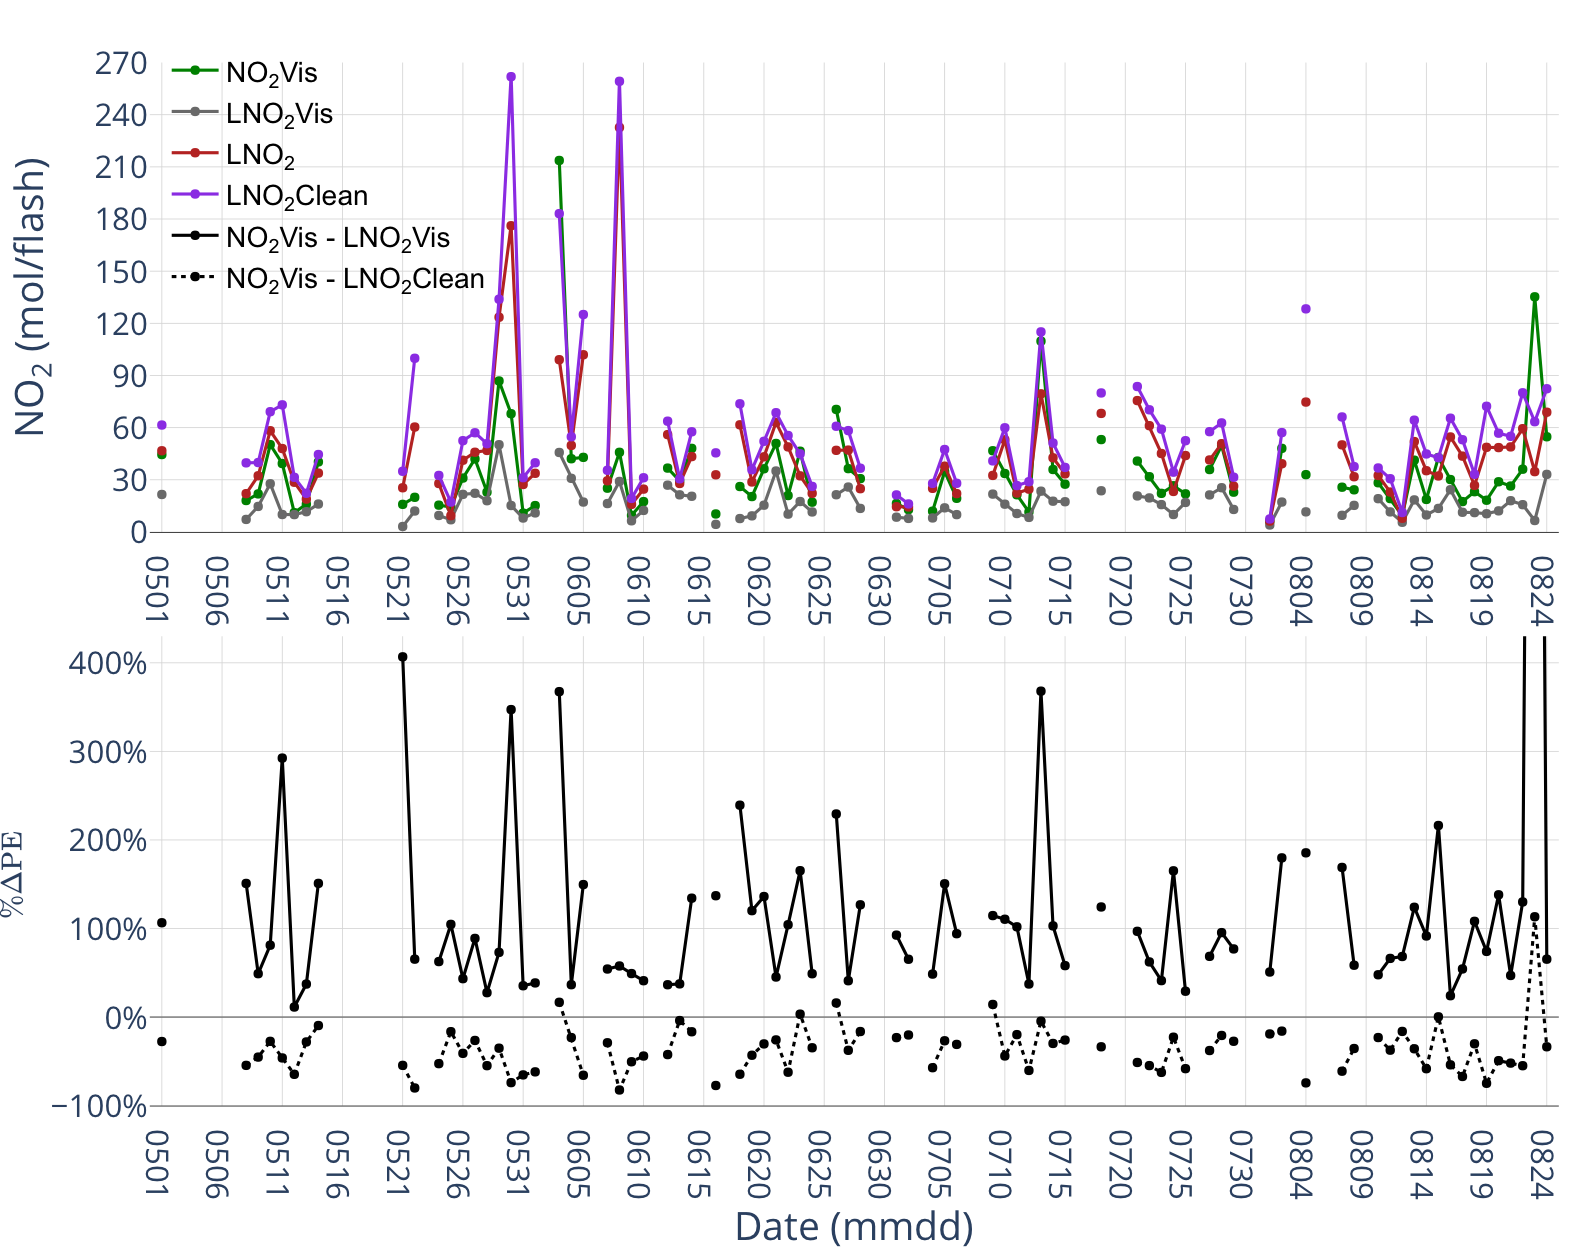
\includegraphics[width=0.9\textwidth]{./figures/us_pe_timeseries.png}
\caption{(上图)2014年5--8月美国大陆的NO$_{\ch{2}}$Vis、LNO$_{\ch{2}}$Vis、LNO$_{\ch{2}}$ 和 LNO$_{\ch{2}}$Clean产率的时间序列,筛选条件为CRF $\geq$ 90\% 和每 2.4 小时 至少2400 次闪电;
(下图)在CRF$\geq$ 90\%的条件下,NO$_{\ch{2}}$Vis 和 LNO$_{\ch{2}}$Vis 之间百分比差异以及 NO$_{\ch{2}}$Vis 和 LNO$_{\ch{2}}$Clean 之间百分比差异的时间序列。
8 月 23 日黑点的值(未显示)为 1958\%。\\
Figure \ref{fig:us_pe_timeseries}. (top) Time series of NO$_{\ch{2}}$Vis, LNO$_{\ch{2}}$Vis, LNO$_{\ch{2}}$ and LNO$_{\ch{2}}$Clean production per day over the CONUS for MJJA 2014 with CRF $\geq$ 90\% and a flash threshold of 2400 flashes per 2.4 h.
(bottom) Time series of the percent differences between NO$_{\ch{2}}$Vis and LNO$_{\ch{2}}$Vis and the percent differences between NO$_{\ch{2}}$Vis and LNO$_{\ch{2}}$Clean with CRF $\geq$ 90\%.
The value of black dot on August 23 (not shown) is 1958\%.}
\label{fig:us_pe_timeseries}
\end{figure}


图\ref{fig:us_pe_linear}为ENTLN 数据与 NO$_{\ch{2}}$Vis、LNO$_{\ch{2}}$Vis、LNO$_{\ch{2}}$ 和 LNO$_{\ch{2}}$Clean摩尔数的线性回归,
其筛选条件与图 \ref{fig:us_pe_timeseries} 相同。
LNO$_{\ch{2}}$Clean 产率为 25.2 $\pm$ 22.3 mol NO$_{\ch{2}}$ 每闪电(相关系数为0.25)
和 2.3 $\pm$ 2.1 mol NO$_{\ch{2}}$每闪击(相关系数为0.22)。
如图\ref{fig:us_pe_timeseries}所示,NO$_{\ch{2}}$Vis产率和LNO$_{\ch{2}}$Clean产率之间的正百分比差异发生的频率远低于负差异的发生频率。
因此,NO$_{\ch{2}}$Vis产率(17.1 $\pm$ 17.2 mol NO$_{\ch{2}}$ 每闪电和0.4 $\pm$ 1.0 mol NO$_{\ch{2}}$ 每闪击)
小于使用线性回归方法得到的 LNO$_{\ch{2}}$Clean产率。


\begin{figure}[H]
\centering
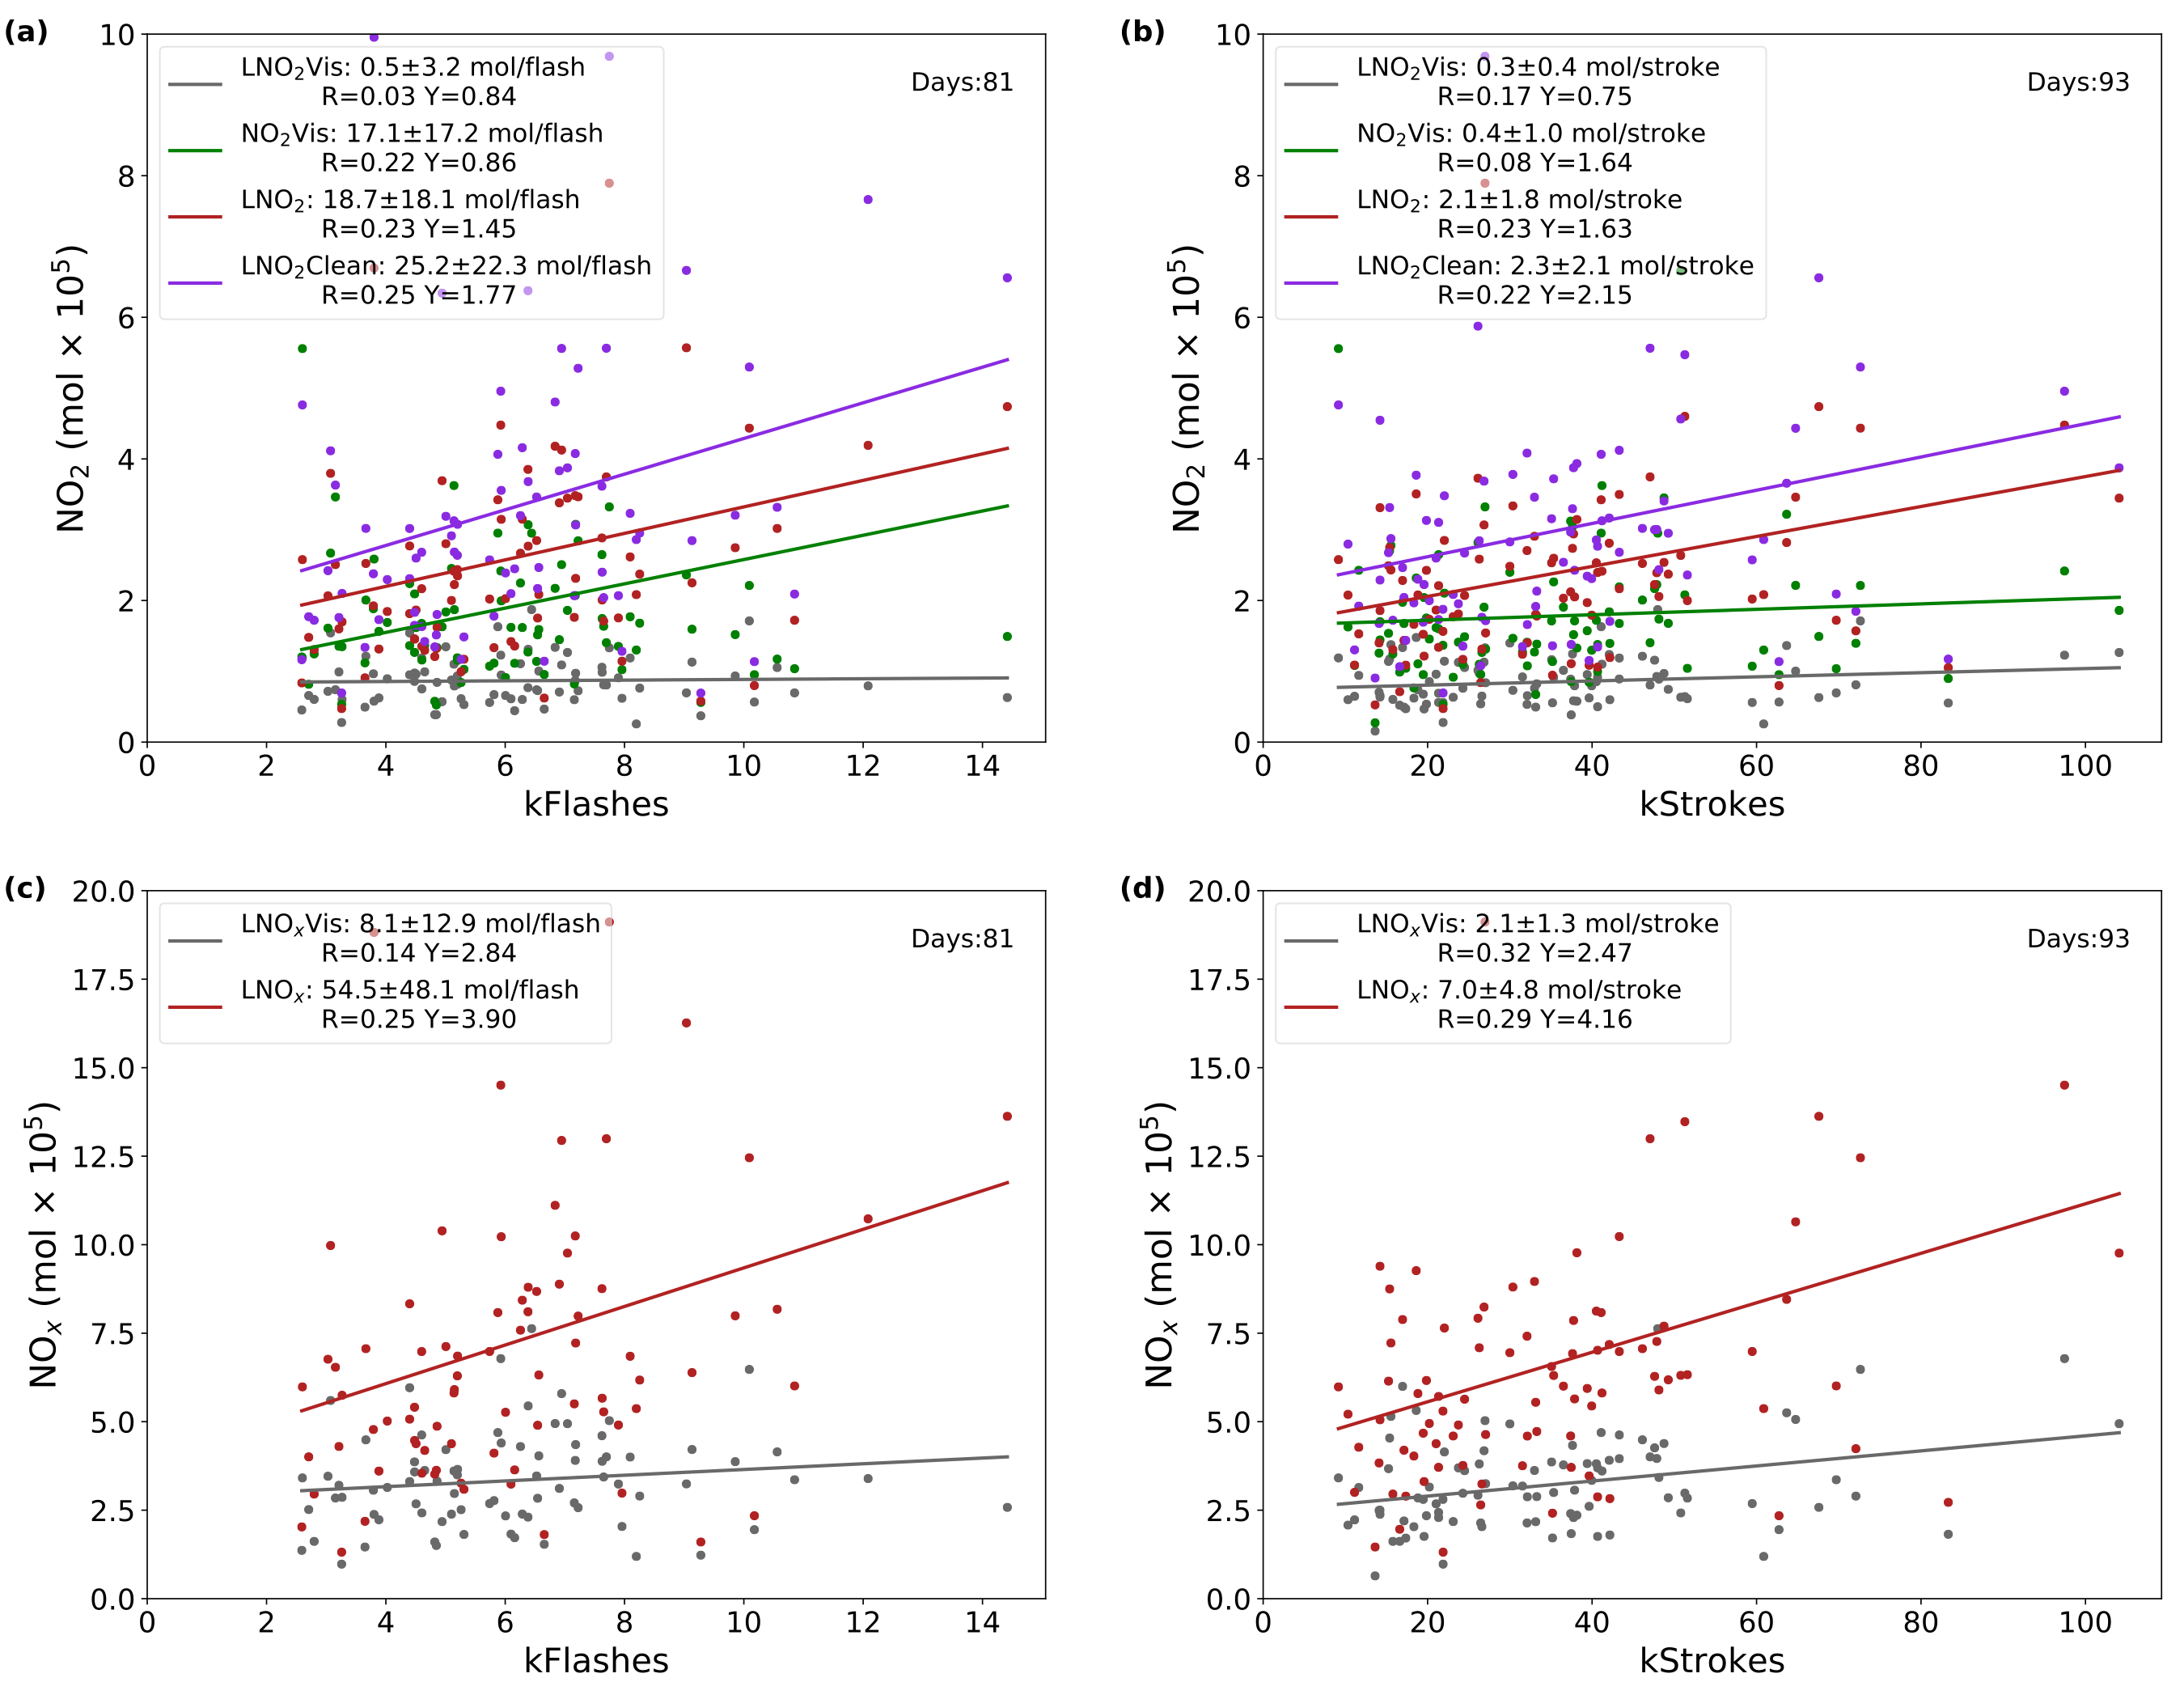
\includegraphics[width=\textwidth]{./figures/us_pe_linear.png}
\caption{(a)每日 NO$_{\ch{2}}$Vis、LNO$_{\ch{2}}$Vis、LNO$_{\ch{2}}$ 和 LNO$_{\ch{2}}$Clean 与 ENTLN 总闪的关系;
(b)与(a)相同,但针对闪击数据;
(c)每日LNO$_{\ch{x}}$Vis 和 LNO$_{\ch{x}}$ 与总闪的关系;
(d)与(c)相同,但针对闪击数据。\\
Figure \ref{fig:us_pe_linear}.
(a) Daily NO$_{\ch{2}}$Vis, LNO$_{\ch{2}}$Vis, LNO$_{\ch{2}}$ and LNO$_{\ch{2}}$Clean versus ENTLN total flashes data.
(b) Same as (a) but for strokes.
(c) Daily LNO$_{\ch{x}}$Vis and LNO$_{\ch{x}}$ versus total flashes.
(d) Same as (c) but for strokes.}
\label{fig:us_pe_linear}
\end{figure}


为了与\citet{Lapierre.2020}的结果进行比较,
本研究选择了CP $\leq$ 650 hPa、TL $\geq$ 1000 和 ratio $\geq$ 50\% 的条件,
然而本研究得到的NO$_{\ch{2}}$Vis(3.8 $\pm$ 0.5 mol每闪击)仍大于\citet{Lapierre.2020}的1.6 $\pm$ 0.1 mol每闪击。
这可能是由两者使用不同版本的伯克利高分辨率(BEHR)算法引起的,\citet{Lapierre.2020}使用的是BEHR v3.0A,本研究的算法基于BEHR v3.0B \citep{Laughner.2019a}。
两个版本中$S_{\ch{NO2}}$均来自于NASA标准产品v3,BEHR v3.0B 的主要改进如下:

(1)使用最接近 OMI 过境时间的廓线,而不是 OMI 过境之前最后一个时刻的廓线;

(2)使用可变的对流层顶高度,而不是固定的200 hPa 对流层顶;

(3)根据\citet{Zhou.2009}的方法计算地表气压。


\begin{figure}[H]
\centering
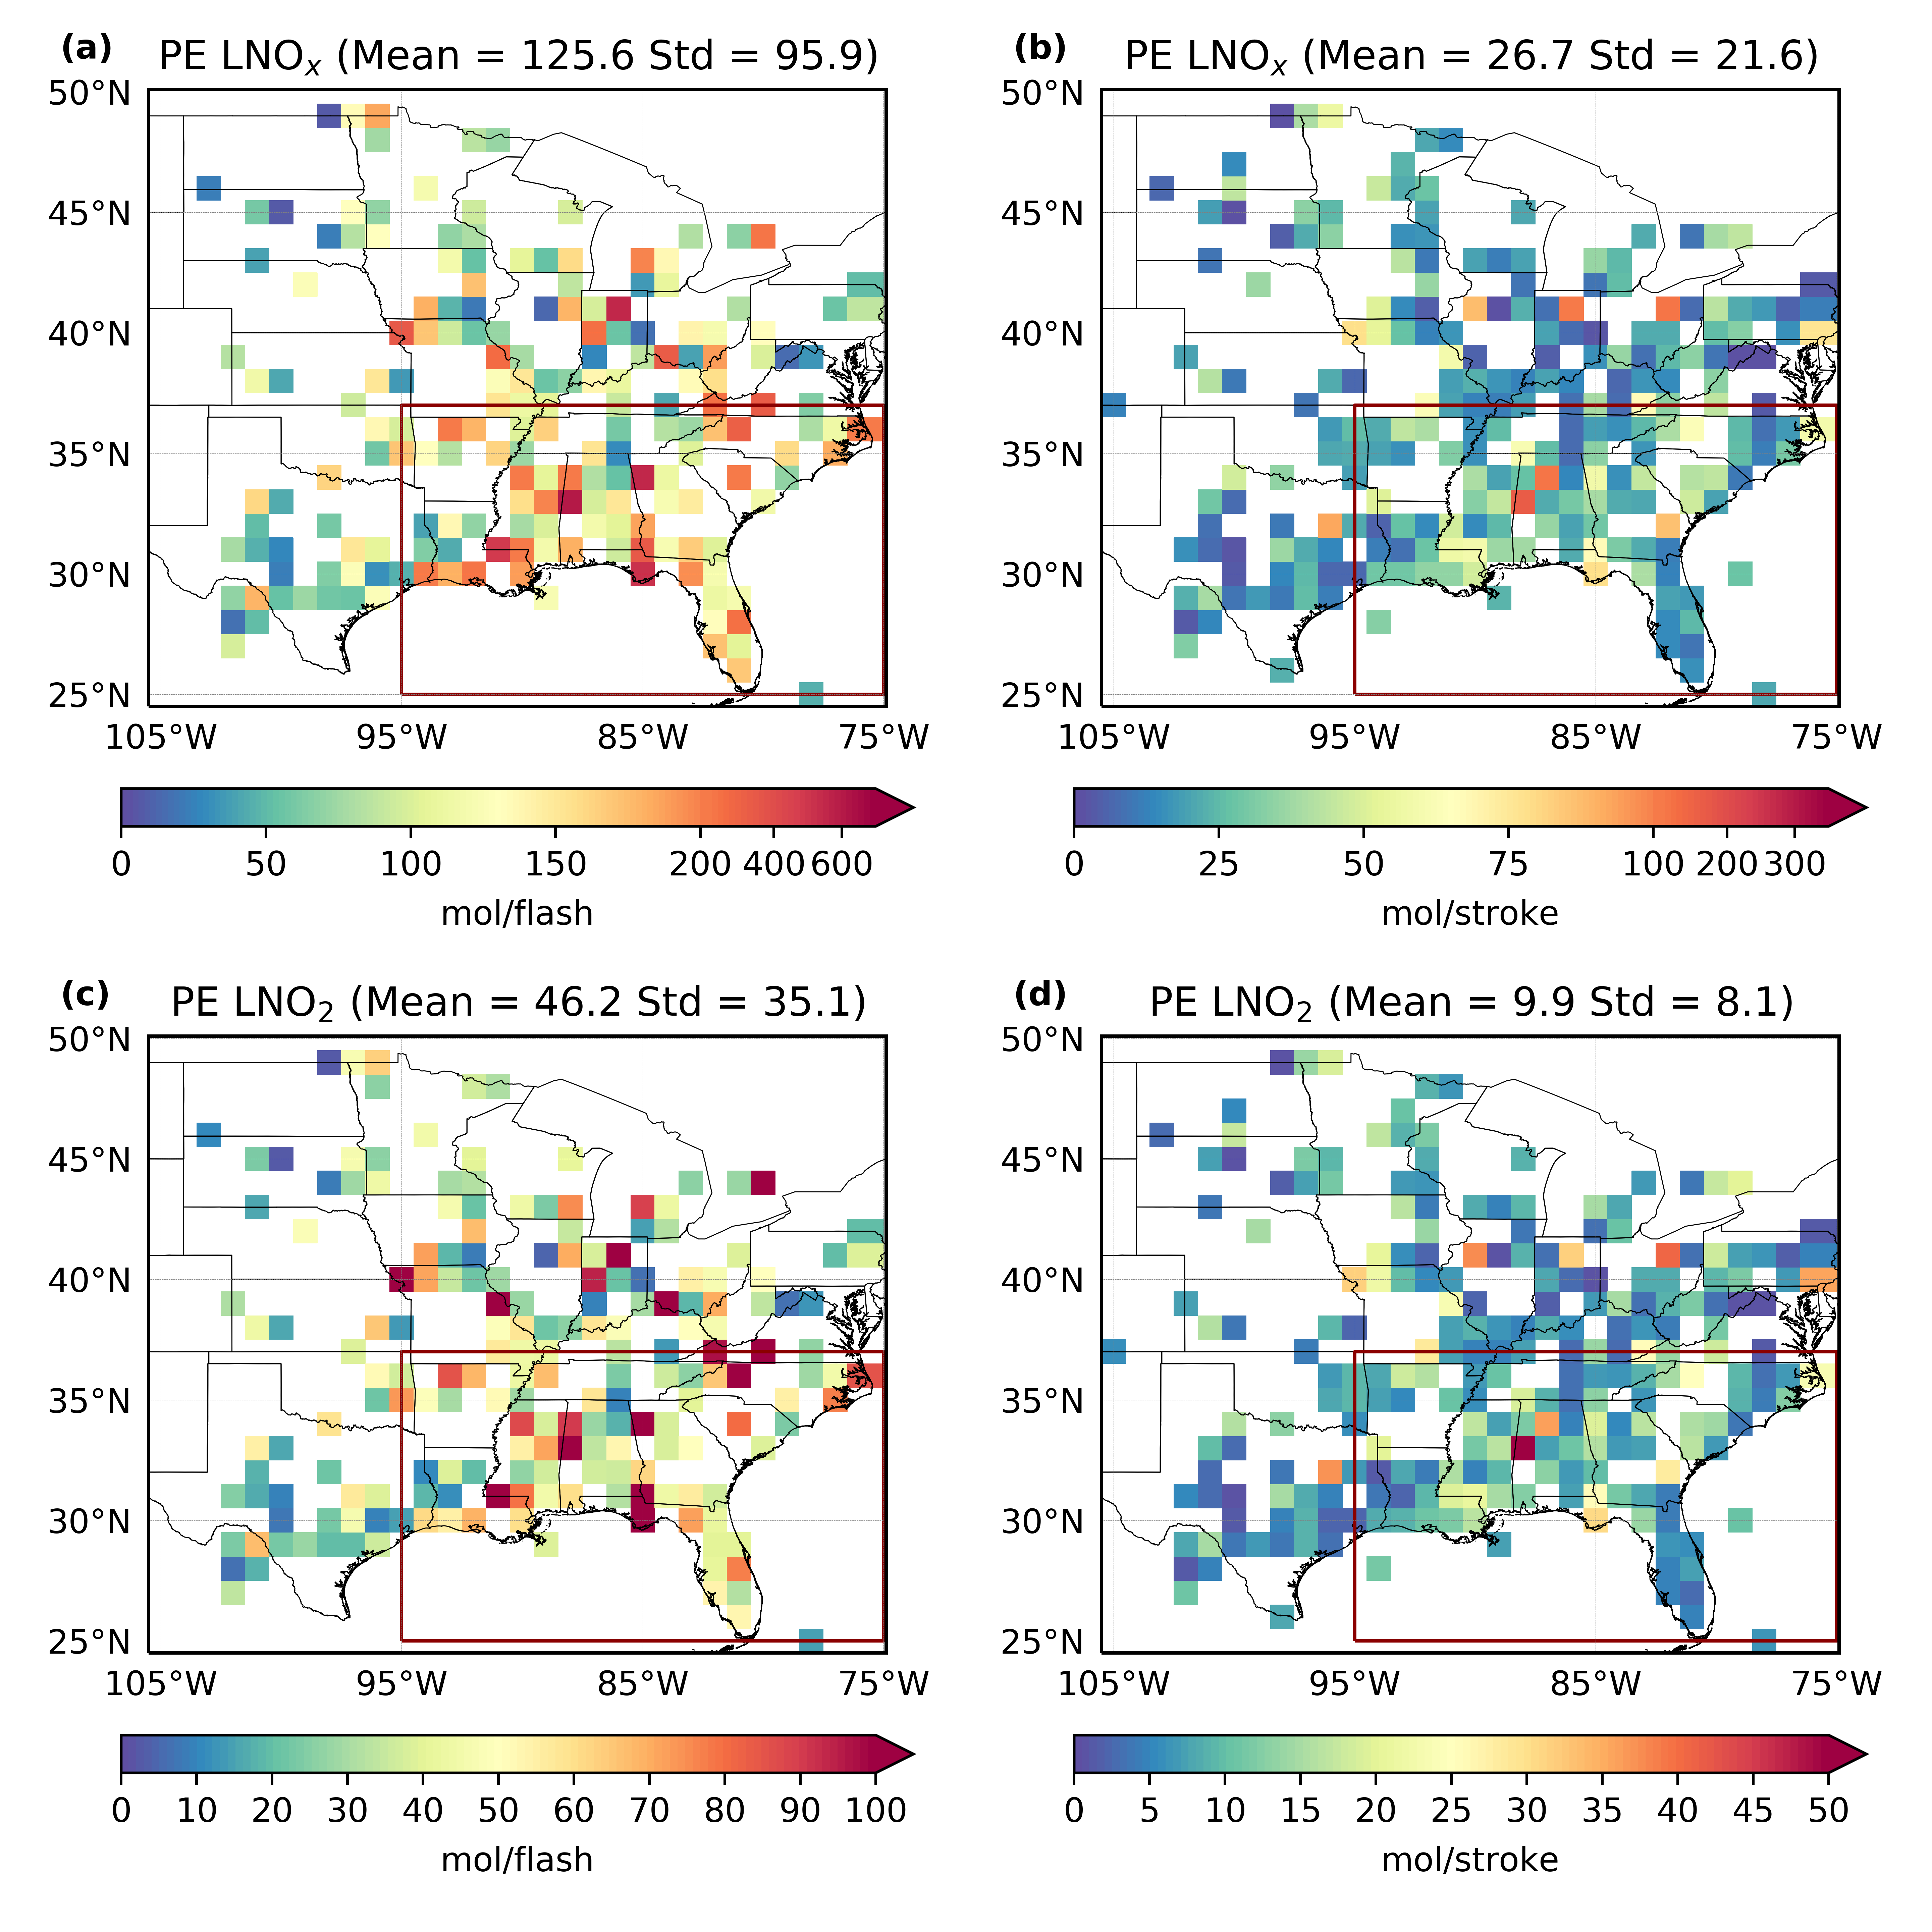
\includegraphics[width=0.95\textwidth]{./figures/us_pe_sum.png}
\caption{(a,c)在CRF $\geq$ 90\%条件下,2014年5--8月 1$^{\circ}$ $\times$ 1$^{\circ}$ LNO$_{\ch{x}}$ 和LNO$_{\ch{2}}$的平均产率分布图;
     (b,d) 与 (a,c) 相同,但针对闪击数据。
     a--d中的红框表示美国东南部。\\
     Figure \ref{fig:us_pe_sum}. (a) and (c) Maps of 1$^{\circ}$ $\times$ 1$^{\circ}$ gridded values of mean LNO$_{\ch{x}}$
    and LNO$_{\ch{2}}$ production per flash with CRF $\geq$ 90\% for MJJA 2014.
    (b) and (d) Same as (a) and (c) except for strokes.
    The southeastern US is denoted by the red box in panels a--d.
}
\label{fig:us_pe_sum}
\end{figure}


% 详细的更新日志见\url{https://github.com/CohenBerkeleyLab/BEHR-core/blob/master/Documentation/Changelog.txt}。
此外,\citet{Lapierre.2020}使用了月平均NO$_{\ch{2}}$廓线,而本研究使用了日廓线,并且将WRF-Chem 输出的间隔调整为 30 min,
这比BEHR 每日产品输出间隔1 h更短,但 AMF 可能还会受到不同 NO$_{\ch{2}}$ 廓线的影响。
鉴于这些因素,本研究在所得数据的基础上来比较不同的方法,以尽量减少这些影响。

结果表明,LNO$_{\ch{2}}$产率(18.7 $\pm$ 18.1 mol每闪电,2.1 $\pm$ 1.8 mol每闪击)介于 LNO$_{\ch{2}}$Clean 和 NO$_{\ch{2}}$Vis产率之间,
与图 \ref{fig:us_pe_timeseries} 中的日结果一致。
此外,基于每日求和值的线性回归结果得到的LNO$_{\ch{x}}$产率为114.8 $\pm$ 18.2 mol每闪电(或17.8 $\pm$ 2.9 mol每闪击),
该结果大于\citet{Pickering.2016}的91 mol每闪电。
这一差异可能是由地理位置、闪电数据和化学模式所共同导致的。
在 CRF $\geq$ 90\% 下,求和法得到LNO$_{\ch{2}}$产率为 46.2 $\pm$ 35.1 mol 每闪电和 9.9 $\pm$ 8.1 mol 每闪击,
而 LNO$_{\ch{x}}$ 产率为 125.6 $\pm$ 95.9 mol 每闪电和 26.7 $\pm$ 21.6 mol 每闪击(图\ref{fig:us_pe_sum})。
其中美国东南部(图\ref{fig:us_pe_sum}中红框,25--37$^{\circ}$ N,75--95$^{\circ}$ W)的 LNO$_{\ch{2}}$和 LNO$_{\ch{x}}$ 产率均较高,这与\citet{Lapierre.2020} 和 \citet{Bucsela.2019}的研究结果相一致。
而与图\ref{fig:us_pe_timeseries}相比,图\ref{fig:us_delta}a--b显示
NO$_{\ch{2}}$Vis产率和 LNO$_{\ch{2}}$Vis产率之间的一些较大差异,这与本研究对污染区域的预期一致。
同时,LNO$_{\ch{2}}$ 和 NO$_{\ch{2}}$Vis产率之间的差异取决于背景 NO$_{\ch{2}}$浓度、上升气流的强度和廓线分布。
负差异是由上升气流携带的背景 NO$_{\ch{2}}$ 污染引起的,
而云下 LNO$_{\ch{2}}$ 的部分导致LNO$_{\ch{2}}$产率高于NO$_{\ch{2}}$Vis产率(图\ref{fig:us_delta}c)。
图\ref{fig:us_delta}d显示 LNO$_{\ch{2}}$Vis在LNO$_{\ch{2}}$中占比为 10--80\%,
这可能是由云层的高度和 LNO$_{\ch{2}}$ 的廓线造成的。
如果云压在300 hPa附近,由于云层的覆盖,该比值将更小。
因此,LNO$_{\ch{x}}$的估算需要更好地了解LNO$_{\ch{2}}$和云下LNO$_{\ch{x}}$的垂直分布。

% \subsection{影响因素及不确定性分析} \label{sec:uncertainty}

图\ref{fig:us_delta}表明,本研究的方法在污染和清洁地区对于LNO$_{\ch{2}}$产率估算的改进程度是不同的。
为了简化量化,本研究选择了CRF = 100\%的条件,具有相似云上NO$_{\ch{2}}$廓线($\sim$ 100 pptv)的六个网格,这样AMF之间的差异取决于较少的参数:
\begin{equation} \label{AMFLNO2_crf100}
AMF_{\ch{LNO2}} = \frac{\int_{p_{\ch{cloud}}}^{p_{\ch{tp}}} w_{\ch{cloudy}}(p) NO_2(p) \: dp}{\int_{p_{\ch{surf}}}^{p_{\ch{tp}}} LNO_2(p) \: dp}
\end{equation}
\begin{equation} \label{AMFNO2Vis_crf100}
AMF_{\ch{NO2Vis}} = \frac{\int_{p_{\ch{cloud}}}^{p_{\ch{tp}}} w_{\ch{cloudy}}(p) NO_2(p) \: dp}{\int_{p_{\ch{cld}}}^{p_{\ch{tp}}} NO_2(p) \: dp}
\end{equation}
\begin{equation} \label{AMFLNO2Clean_crf100}
AMF_{\ch{LNO2Clean}} = \frac{\int_{p_{\ch{cloud}}}^{p_{\ch{tp}}} w_{\ch{cloudy}}(p) LNO_2(p) \: dp}{\int_{p_{\ch{surf}}}^{p_{\ch{tp}}} LNO_2(p) \: dp}
\end{equation}
这些网格框包含图\ref{fig:us_delta}a中的污染城市(星形)和清洁城市(三角形)。
图\ref{fig:us_bkgd_comp}比较了污染和清洁网格内NO$_{\ch{2}}$、背景 NO$_{\ch{2}}$ 和背景 NO$_{\ch{2}}$占比的平均廓线。
由于对流层上层LNO$_{\ch{2}}$ 浓度高于背景 NO$_{\ch{2}}$ 浓度,背景 NO$_{\ch{2}}$ 与总 NO$_{\ch{2}}$ 的比例曲线呈 C 形。
然而随着背景 NO$_{\ch{2}}$ 增加和 LNO$_{\ch{2}}$ 的减少,图\ref{fig:us_bkgd_comp}e中的比例在云压和对流层顶之间存在峰值。
此外污染地区的对流层上层背景NO$_{\ch{2}}$占比稳定且高于清洁地区。

表\ref{table:production_comp}显示了对于6个城市三种方法之间的相对变化。
AMF$_{\ch{LNO2}}$(式\ref{AMFLNO2_crf100})和 AMF$_{\ch{LNO2Clean}}$(式\ref{AMFLNO2Clean_crf100})之间的区别是分子:
$\int_{p_{\ch{cloud}}}^{p_{\ch{tp}}} w_{\ch{cloudy}}(p) NO_2(p) \: dp$
和$\int_{p_{\ch{cloud}}}^{p_{\ch{tp}}} w_{\ch{cloudy}}(p) LNO_2(p) \: dp$。
当 LNO$_{\ch{2}}$ 的比例较高或区域较清洁时,两者相对差异较小(5.0--12.0\%,图\ref{fig:us_bkgd_comp}d--f),
最大的相对差异(46.3\%)发生在对流层上层背景 NO$_{\ch{2}}$ 所占比例一直较高的情况下(图\ref{fig:us_bkgd_comp}c)。
因此本研究的反演方法对背景 NO$_{\ch{2}}$ 不太敏感,更适用于受污染地区的对流情况。
相比之下,由于包含了云层下方的 LNO$_{\ch{2}}$,本研究估算的产量大于基于 NO$_{\ch{2}}$Vis 的产量。
当云层较高时,特别是 LNO廓线的峰值低于云层时(图\ref{fig:us_bkgd_comp}b),
相对差异较大(121.2\%),因为更多的 LNO$_{\ch{2}}$ 不能包含在 NO$_{\ch{2}}$Vis 中。
AMF$_{\ch{LNO2Clean}}$(式\ref{AMFLNO2Clean_crf100})和 AMF$_{\ch{NO2Vis}}$(式\ref{AMFNO2Vis_crf100})之间的相对变化取决于
$\int_{p_{\textrm cloud}}^{p_{\textrm tp}} w_{\textrm cloudy}(p) LNO_2(p) \: dp / \int_{p_{\textrm surf}}^{p_{\textrm tp}} w_{\textrm cloudy}(p) LNO_2(p) \: dp$,这也是受云影响,而不是背景NO$_{\ch{2}}$。
其中最大的相对变化(153.8\%)发生在新奥尔良,它的云压最小(云层最高),因此可见的柱浓度最小。


\begin{table}[H]
\caption{基于相同先验廓线但不同估算方法时,产量的百分比变化\\Table \ref{table:production_comp}. The percent changes in the estimated production when using different methods based on the same a priori profiles.}
\scriptsize
\centering
\begin{tabular}{clccc}
\thickline
 & 城市$^a$ & (LNO$_{\ch{2}}$Clean - LNO$_{\ch{2}}$)/LNO$_{\ch{2}}$ & (LNO$_{\ch{2}}$ - TropVis)/TropVis & (LNO$_{\ch{2}}$Clean-TropVis)/TropVis \\
\thickline
\multirow{3}{*}{污染地区} & Lansing          & 24.2\%  & 49.5\%   & 85.6\%   \\
                         & New Orleans      & 13.3\%  & 121.2\%  & 153.8\%  \\
                         & Orlando          & 46.3\%  & 37.5\%   & 101.3\%  \\
\hline
\multirow{3}{*}{清洁地区}    & Huron            & 12.0\%  & 56.4\%   & 75.2\%   \\
                            & Charles Town     & 12.0\%  & 82.2\%   & 104.1\%  \\
                            & Tarboro          & 5.0\%   & 86.0\%   & 95.3\%   \\
\thickline
\end{tabular}
\begin{tablenotes}
\linespread{1}\footnotesize
\item $^a$城市地址见图\ref{fig:us_delta}a。
\item $^a$Locations are denoted in Fig. \ref{fig:us_delta}a.
\end{tablenotes}
\label{table:production_comp}
\end{table}

图\ref{fig:us_cp_ratio_lno2}a为2014年5--8月在CRF$\geq$90\%的条件下,云压和$V_{\ch{LNO2Vis}}$与$V_{\ch{LNO2}}$之比的日分布。
当云压从600降低到300 hPa时,$V_{\ch{LNO2Vis}}$与$V_{\ch{LNO2}}$之比从 0.8 降低到 0.2,
故在相对清洁的区域,NO$_{\ch{2}}$Vis产率小于LNO$_{\ch{2}}$产率。
除了 LNO$_{\ch{2}}$Vis,LNO$_{\ch{2}}$产率也是受云压影响。
对于大于 30 mol每闪击的LNO$_{\ch{2}}$产率,云压均小于 550 hPa(图\ref{fig:us_cp_ratio_lno2}b),
而较小的 LNO$_{\ch{2}}$ 产率(<30 mol每闪击)出现在 650 hPa 和 200 hPa 之间。
由于较高的LNO$_{\ch{2}}$ 产率和闪电数据数量有限,现阶段本研究无法推出 LNO$_{\ch{2}}$ 产率与云压或其他闪电属性之间的关系。
由于云压仅代表云的发展,因此不能仅从云压值推导出闪电的垂直结构。
前人研究表示,不同闪电的闪电通道长度会有所不同,并且取决于环境条件\citep{Carey.2016,Mecikalski.2017,Fuchs.2018}。
\citet{Davis.2019}比较了两种闪电:正常闪电和异常闪电。
一般来说,正常闪电是上层带正电和中层带负电,而异常闪电则相反\citep{Williams.1989}。
由于异常闪电中上升气流更强且闪电频率更高,因此异常闪电的对流层上层LNO$_{\ch{x}}$浓度高于正常闪电。


\begin{figure}[H]
\centering
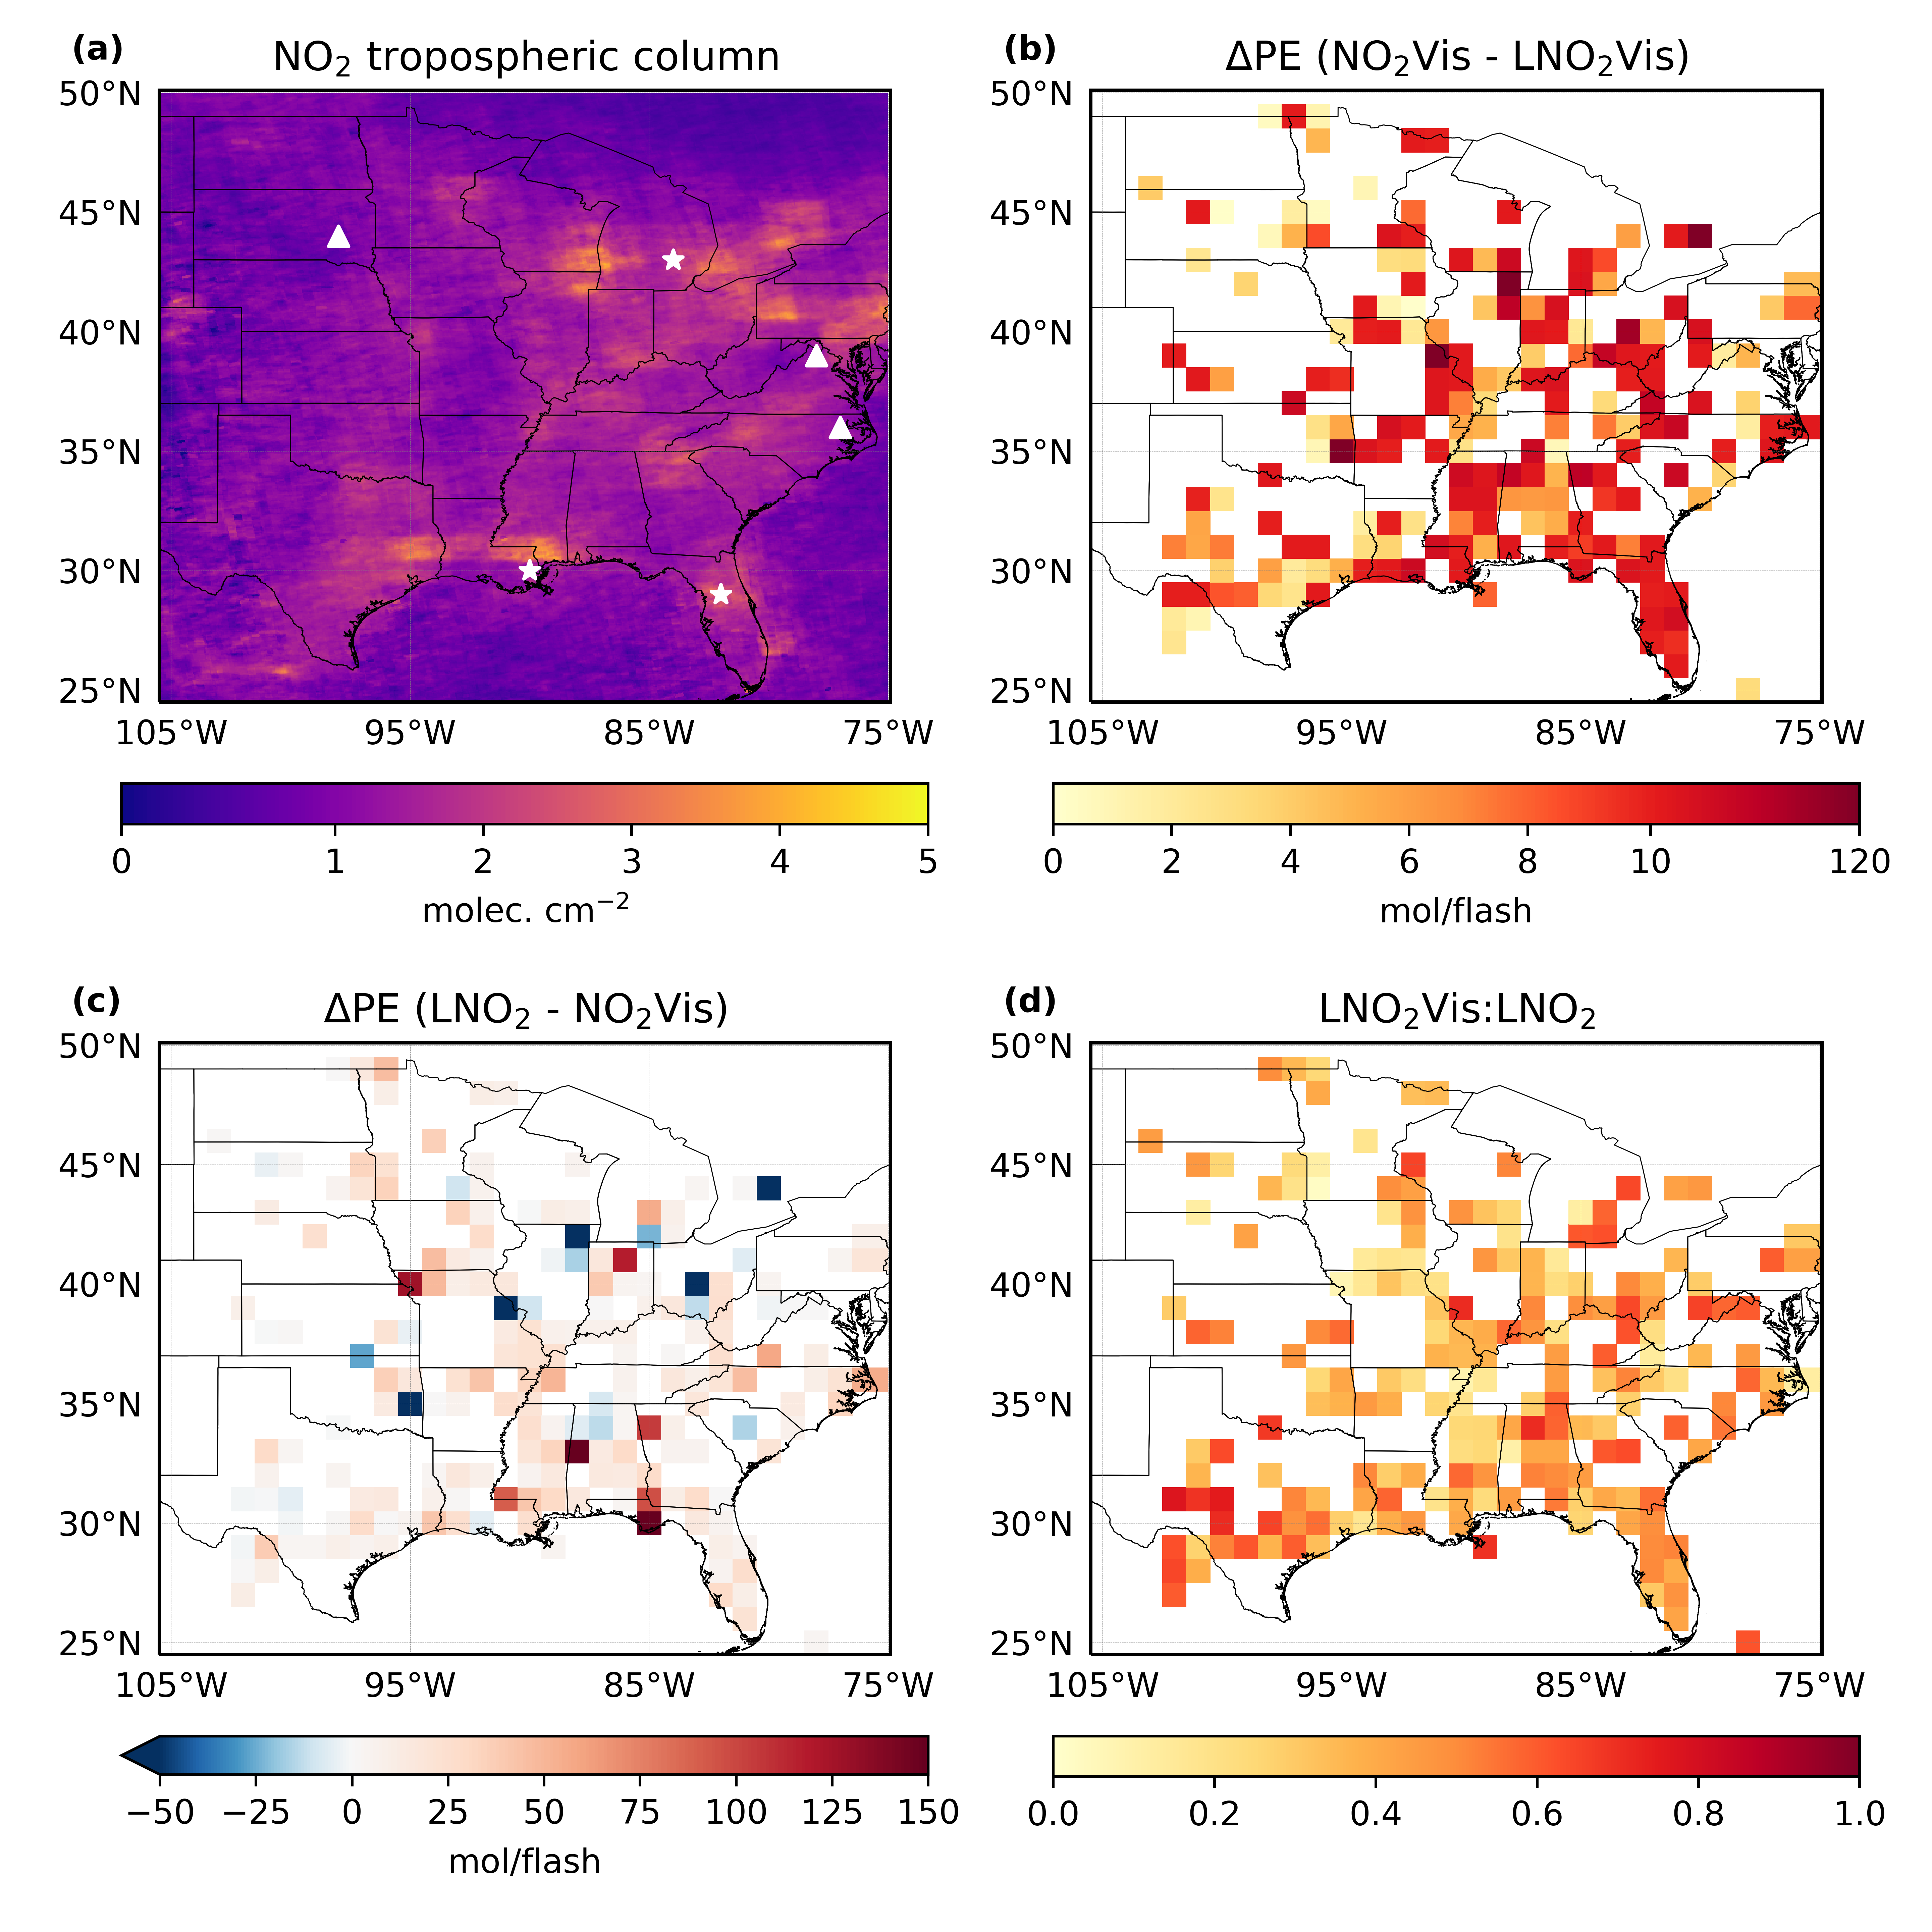
\includegraphics[width=0.95\textwidth]{./figures/us_delta.png}
\caption{(a)2014年5--8月平均对流层NO$_{\ch{2}}$柱浓度,
污染城市用星号表示:兰辛、新奥尔良和奥兰多,而清洁城市用三角形表示:休伦、查尔斯镇和塔伯勒;
(b)在CRF $\geq$ 90\%条件下,NO$_{\ch{2}}$Vis 和 LNO$_{\ch{2}}$Vis平均产率的差异;
(c)与(b)相同,但为 LNO$_{\ch{2}}$ 和 NO$_{\ch{2}}$Vis 之间的差异;
(d)LNO$_{\ch{2}}$Vis 与 LNO$_{\ch{2}}$ 的比例。\\
Figure \ref{fig:us_delta}.
(a) Mean NO$_{\ch{2}}$ tropospheric column for MJJA 2014.
Polluted cities are denoted by stars: Lansing, New Orleans and Orlando, while clean cities are denoted by triangles: Huron, Charles Town and Tarboro.
(b) The differences of the estimated mean production efficiency between NO$_{\ch{2}}$Vis and LNO$_{\ch{2}}$Vis with CRF $\geq$ 90\%.
(c) The same differences as (b) but between LNO$_{\ch{2}}$ and NO$_{\ch{2}}$Vis.
(d) The ratio of LNO$_{\ch{2}}$Vis to LNO$_{\ch{2}}$.
}
\label{fig:us_delta}
\end{figure}


\begin{landscape}
\clearpage\vspace*{\fill}
% \begin{sidewaysfigure}[htbp!]
\begin{figure}[!ht]
\centering
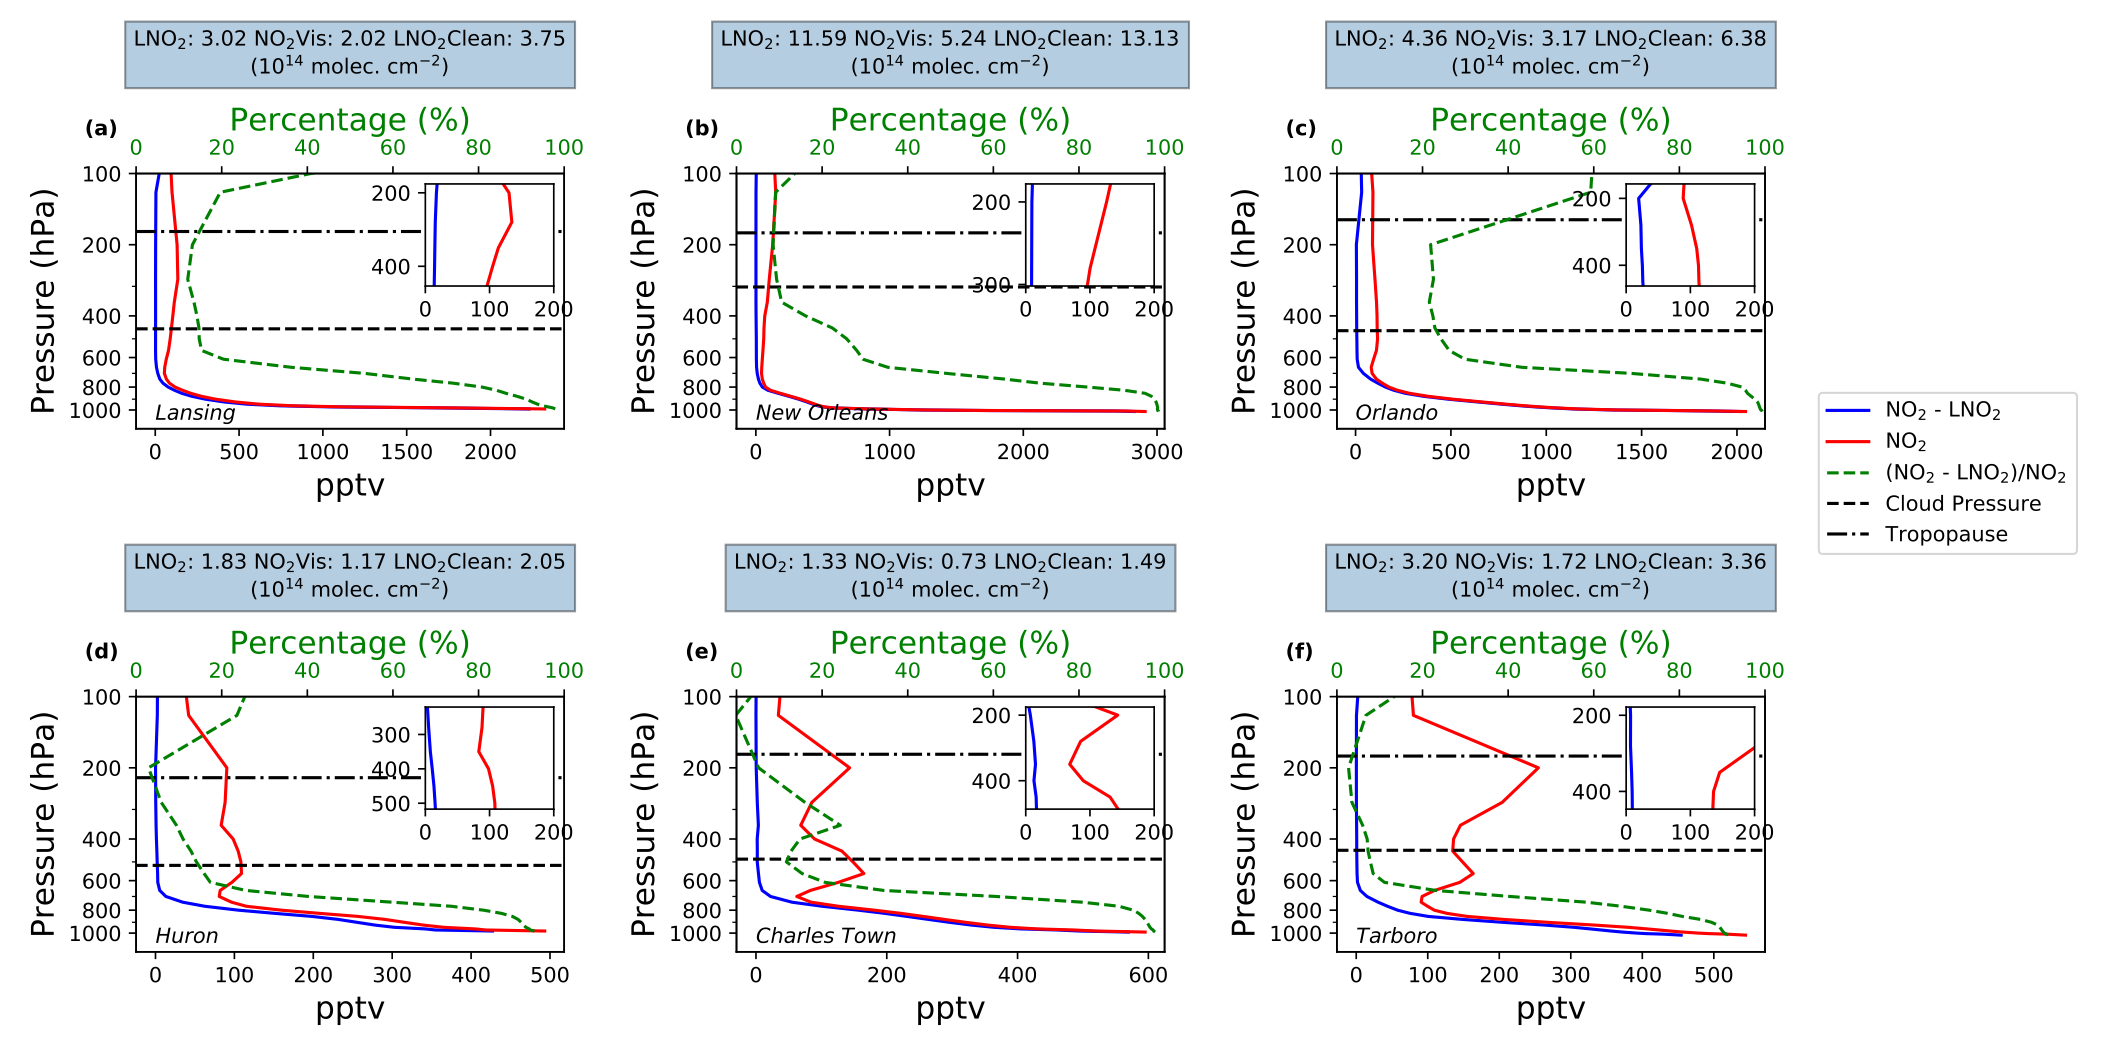
\includegraphics[width=0.85\columnwidth]{./figures/us_bkgd_comp.png}%
% 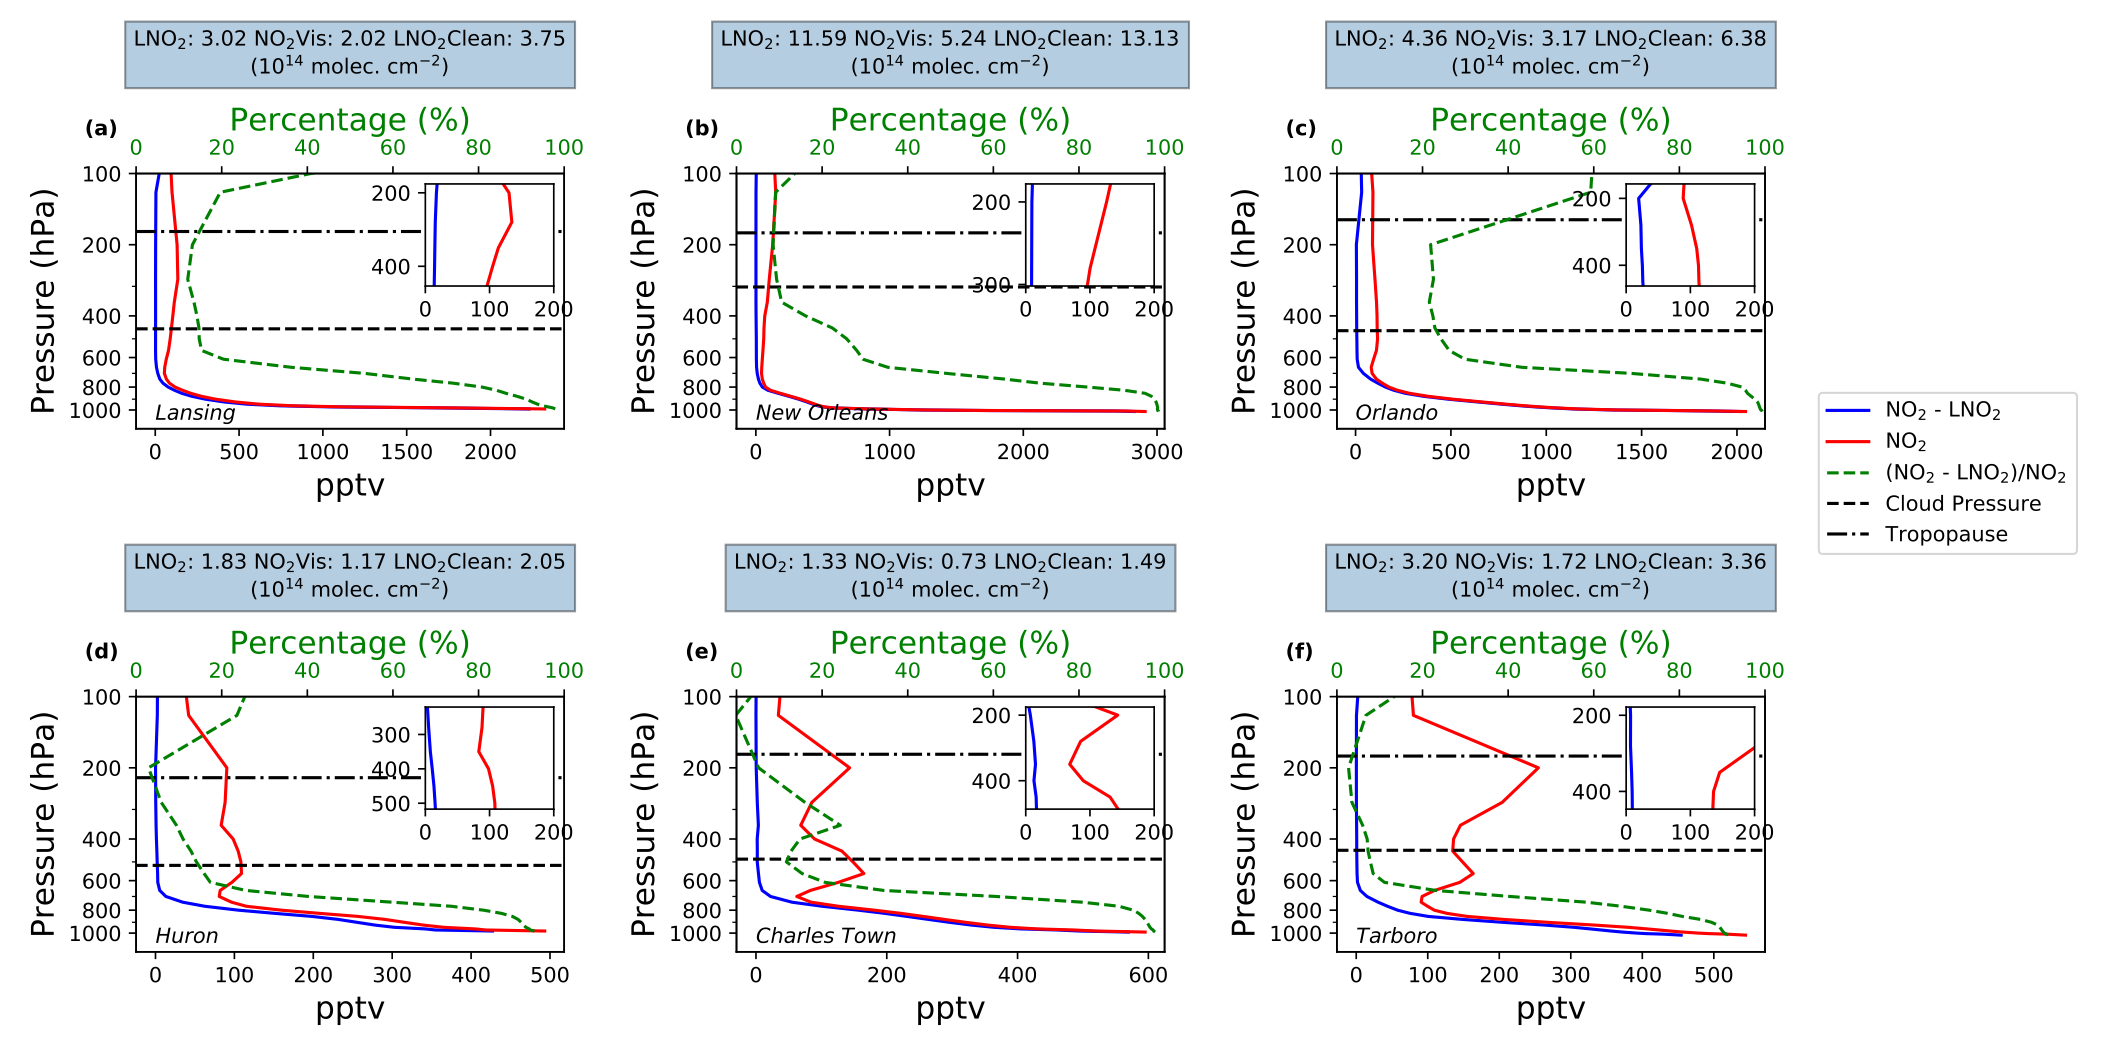
\includegraphics[width=\textwidth]{./figures/us_bkgd_comp.png}%
\caption{CRF $\geq$ 100\%条件下,六个网格中WRF-Chem 平均NO$_\textrm{2}$ 和背景 NO$_\textrm{2}$ 廓线。
顶行数据选自污染区域(图 \ref{fig:us_delta}a中星形),而底行数据来自清洁区域(图 \ref{fig:us_delta}a中三角形)。
绿色虚线是背景 NO$_\textrm{2}$占比的廓线,
放大图显示了从云压到对流层顶的廓线。
标题为基于\ref{sec:amf_definition}节定义的三种不同方法估算得到的产量。\\
Figure \ref{fig:us_bkgd_comp}. Comparisons of mean WRF-Chem NO$_\textrm{2}$ and background NO$_\textrm{2}$ profiles in six grids with CRF $\geq$ 100\%.
The top row data are selected from polluted regions (stars in Fig. \ref{fig:us_delta}a) while the bottom row data are from clean regions (triangles in Fig. \ref{fig:us_delta}a).
The green dashed lines are the mean ratio profiles of background NO$_\textrm{2}$ to total NO$_\textrm{2}$.
The zoomed figures show the profiles from the cloud pressure to the tropopause.
The titles present the mean productions based on three different methods mentioned in Sect. \ref{sec:amf_definition}.}
\label{fig:us_bkgd_comp}
% \end{sidewaysfigure}
\end{figure}
\vspace*{\fill}\clearpage
\end{landscape}

% \vspace{5mm}
\begin{figure}[H]
\centering
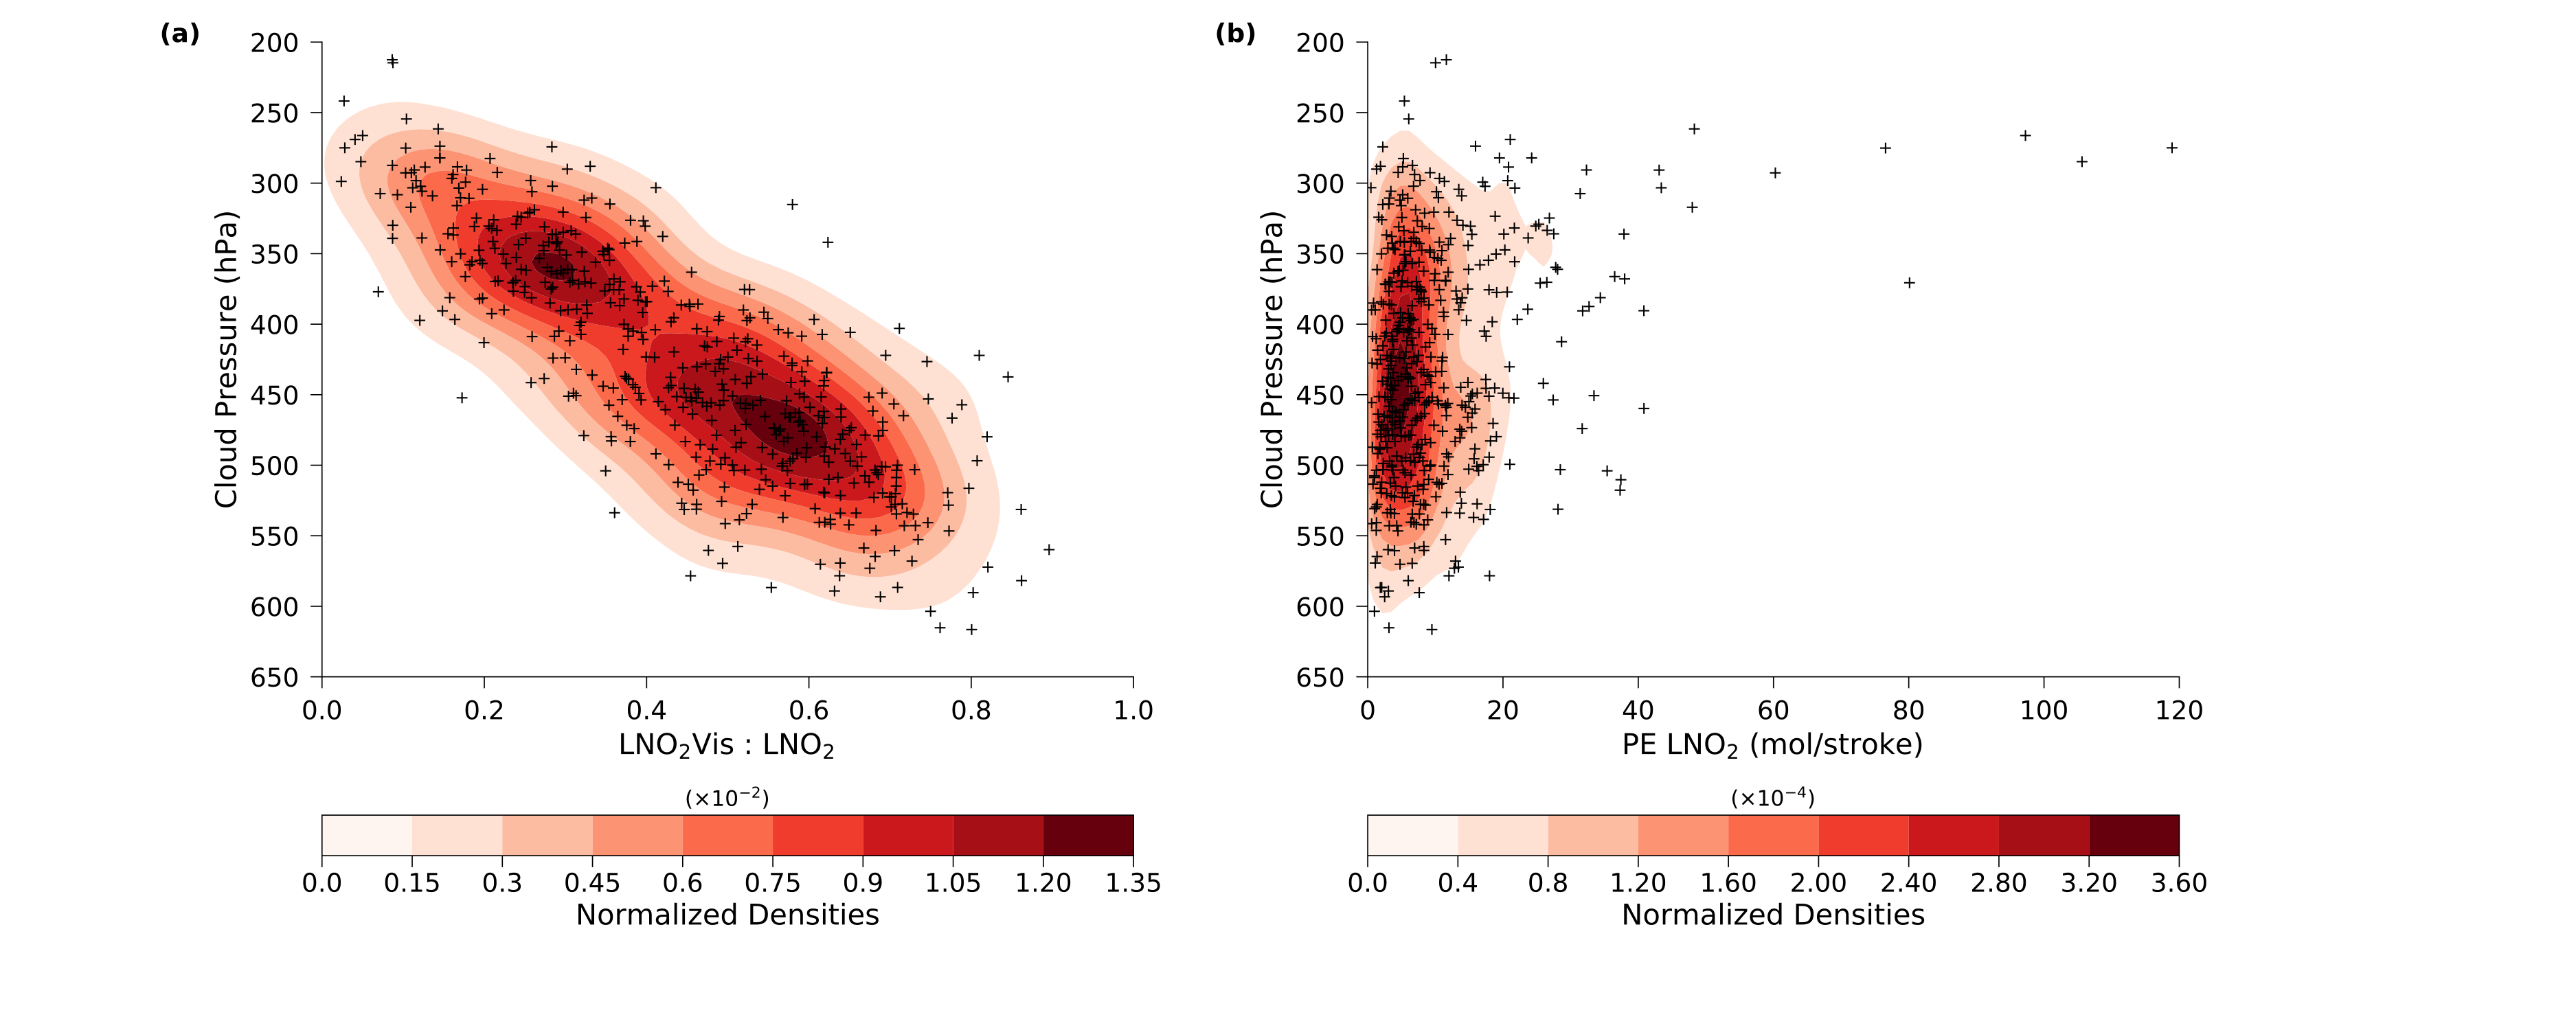
\includegraphics[width=\textwidth]{./figures/us_cp_ratio_lno2.png}
\caption{(a)$V_{\ch{LNO2Vis}}$与$V_{\ch{LNO2}}$之比的核密度估计;(b)LNO$_{\ch{2}}$产率与OMI测得云压的核密度估计(2014年5--8月,CRF $\geq$ 90\%)。\\
Figure \ref{fig:us_cp_ratio_lno2}. Kernel density estimation of the (a) daily ratio of $V_{\ch{LNO2Vis}}$ to $V_{\ch{LNO2}}$ and (b) daily LNO$_{\ch{2}}$ production efficiency (PE) versus the daily cloud pressure measured by OMI with CRF $\geq$ 90\% for MJJA 2014.}
\label{fig:us_cp_ratio_lno2}
\end{figure}
% \vspace{5mm}



% \subsection{闪电氮氧化物产率与云属性和闪电参数化之间的关系}

\subsection{反演及产率计算中的不确定性分析}


% 模式中LNO$_{\ch{x}}$的分布主要有两种方法:已通过对流输送重新分布的LNO$_{\ch{x}}$廓线(对流后)和在对流输送重新分布之前LNO$_{\ch{x}}$的廓线(对流前)\citep{Allen.2012,Luo.2017}。
% 然而,鉴于与其他 LNO$_{\ch{x}}$ 研究相比结果的相似性,我们相信本文研究中基于对流后LNO$_{\ch{x}}$廓线的1$^{\circ}$ $\times$ 1$^{\circ}$结果足以估计LNO$_{\ch{x}}$的平均产量。
WRF-Chem中LNO排放的设置在不同的研究中有所不同。
\citet{Zhao.2009}在区域尺度模式中将NO产率设定为250 mol NO每闪电,
而 \citet{Bela.2016}选择了\citet{Barth.2012}使用的330 mol NO每闪电。
\citet{Wang.2015a}假设每次闪电产生大约 500 mol NO,这是通过云尺度化学传输模式和云中飞机观测得出的\citep{Ott.2010}。
为了评估 LNO$_{\ch{2}}$参数化对 LNO$_{\ch{2}}$估算的影响,
本研究将WRF-Chem 基于另一个LNO设置(2$\times$基本闪率,500 mol NO每闪电,以下简称“2$\times$500 mol NO每闪电”)的NO$_{\ch{2}}$模拟结果
应用于先验廓线,并评估 AMF$_{\ch{LNO$_2$}}$、AMF$_{\ch{LNO$_x$}}$、LNO$_{\ch{2}}$产率和 LNO$_{\ch{x}}$产率相对于1$\times$200 mol NO 每闪电所得结果的变化。
对于线性回归方法(图 \ref{fig:us_pe_linear_2x500}),LNO$_{\ch{2}}$产率为 29.8 $\pm$ 20.5 mol每闪电,
比基本设置所得结果(18.7 $\pm$ 18.1 mol每闪电)大59.4\%,
与此同时LNO$_{\ch{x}}$产率(从54.5 $\pm$ 48.1 mol每闪电增加到88.5 $\pm$ 61.1 mol每闪电)也取决于 WRF-Chem 中 LNO产率的设置。
通过比较图\ref{fig:us_pe_linear}和图\ref{fig:us_pe_linear_2x500},结果表明当LNO$_{\ch{2}}$和NO$_{\ch{2}}$Vis产率呈现相同趋势时,
LNO$_{\ch{2}}$Clean和 LNO$_{\ch{2}}$产率更相似。
% 目前尚不清楚 NO--NO$_{\ch{2}}$--O$_{\ch{3}}$ 循环或其他 LNO$_{\ch{x}}$ 汇对LNO$_{\ch{x}}$产率变化的贡献,
% 这需利用 WRF-Chem进行详细的来源解析,超出了目前本研究的范围。


图\ref{fig:us_simulation_diff}显示了基于 1$\times$200 和 2$\times$500 mol NO 每闪电得到的AMF$_\textrm{LNO$_{\ch{2}}$}$、AMF$_\textrm{LNO$_{\ch{x}}$}$、LNO$_{\ch{2}}$和 LNO$_{\ch{x}}$ 的平均百分比变化。
更高的LNO产率设置对LNO$_{\ch{2}}$和 LNO$_{\ch{x}}$的影响趋势相同:较小的AMF$_\textrm{LNO$_{\ch{2}}$}$和AMF$_\textrm{LNO$_{\ch{x}}$}$导致较大的LNO$_{\ch{2}}$和 LNO$_{\ch{x}}$,但变化幅度具有区域性。
这是由AMF$_\textrm{LNO$_{\ch{2}}$}$和AMF$_\textrm{LNO$_{\ch{x}}$}$的非线性计算引起的。
随着LNO$_{\ch{2}}$的贡献增大,AMF方程式的分子和分母都增大。
因为LNO$_{\ch{2}}$只占云上NO$_{\ch{2}}$的一小部分,分母增加的幅度可能与分子增加的幅度不同,从而对AMF$_\textrm{LNO$_{\ch{2}}$}$和AMF$_\textrm{LNO$_{\ch{x}}$}$产生不同的影响。
如\citet{Zhu.2019}所述,使用 2$\times$500 mol NO 每闪电的设置和与本研究相同的闪电参数化可能会高估美国东南部的闪电密度。
幸运的是,该地区的 AMF 和估算得到的LNO$_{\ch{2}}$变化不大。
由于美国东南部的闪电密度最高,AMF 分子中的NO$_{\ch{2}}$以LNO$_{\ch{2}}$为主,
当模式使用较高的LNO$_{\ch{2}}$时,分子和分母增幅相当。
换言之,对 LNO 设置的敏感性低,LNO$_{\ch{2}}$的相对分布很重要。


\vspace{5mm}
\begin{figure}[H]
\centering
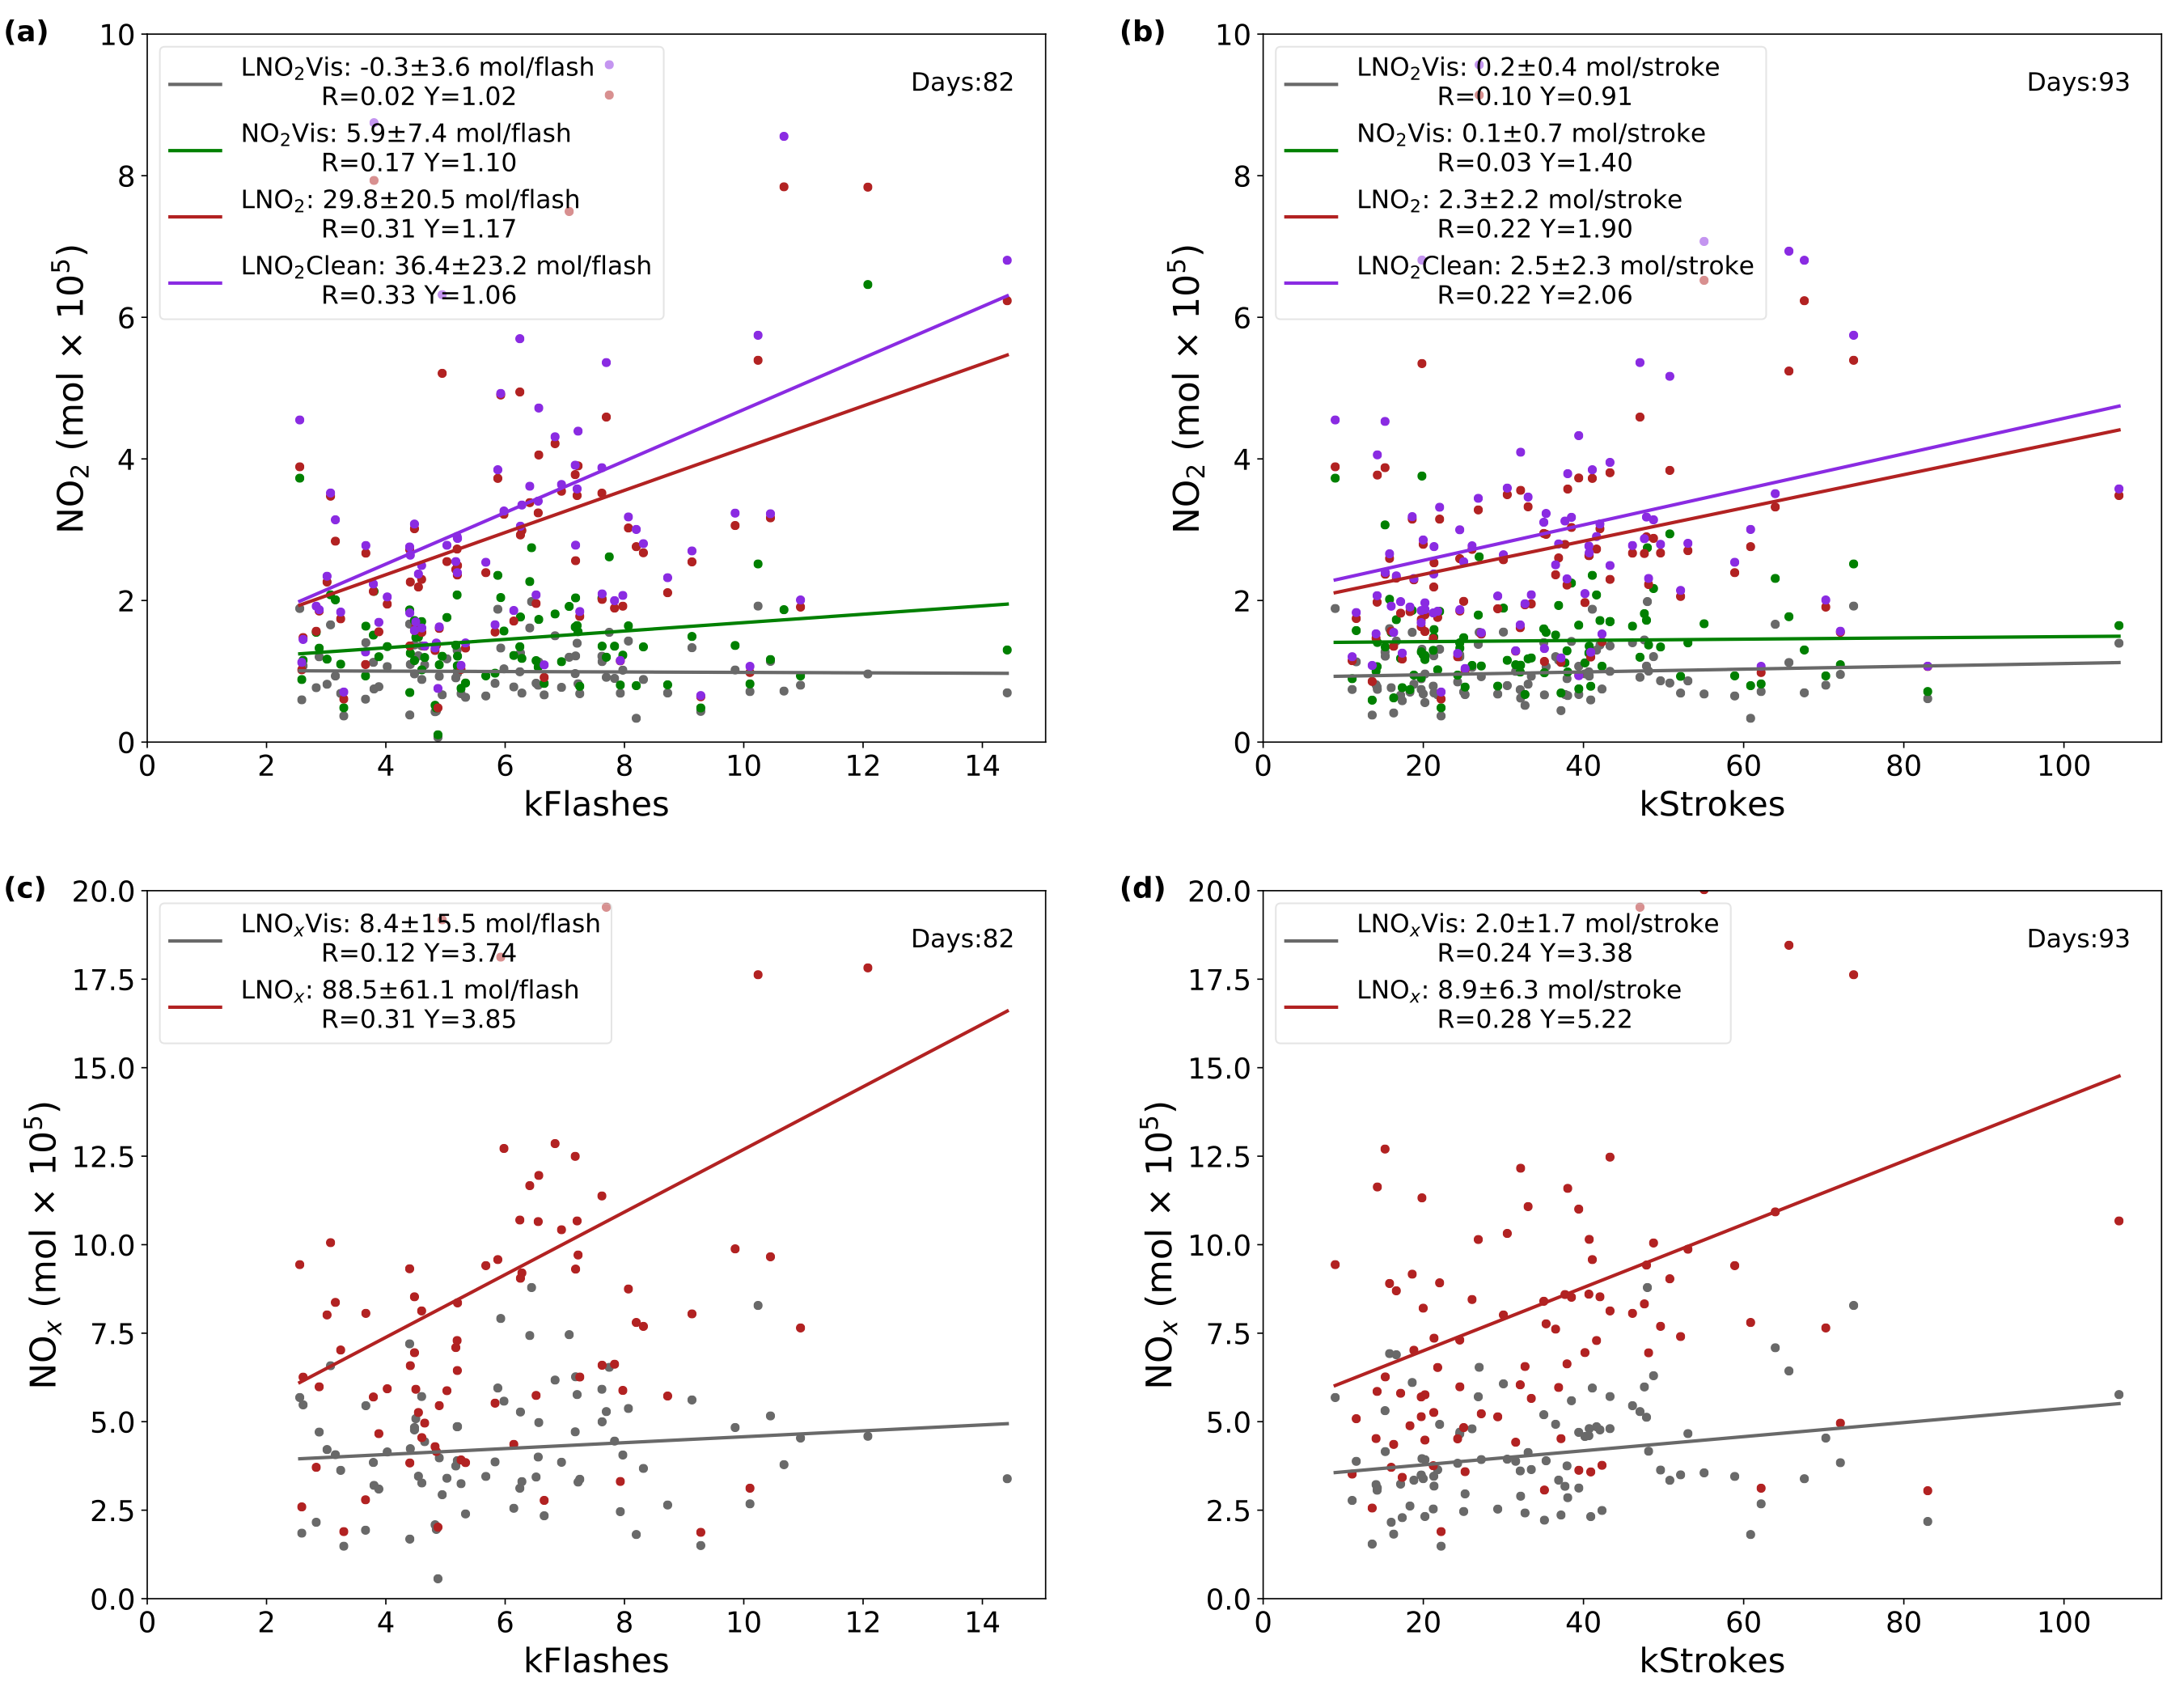
\includegraphics[width=\textwidth]{./figures/us_pe_linear_2x500.png}
\caption{与图\ref{fig:us_pe_linear}相同,但是模式中NO产率设置为2$\times$500 mol每闪电 \\Figure \ref{fig:us_pe_linear_2x500}. Same as Fig. \ref{fig:us_pe_linear} except for the 2$\times$500 mol NO flash$^{-1}$ configuration.}
\label{fig:us_pe_linear_2x500}
\end{figure}

\begin{figure}[H]
\centering
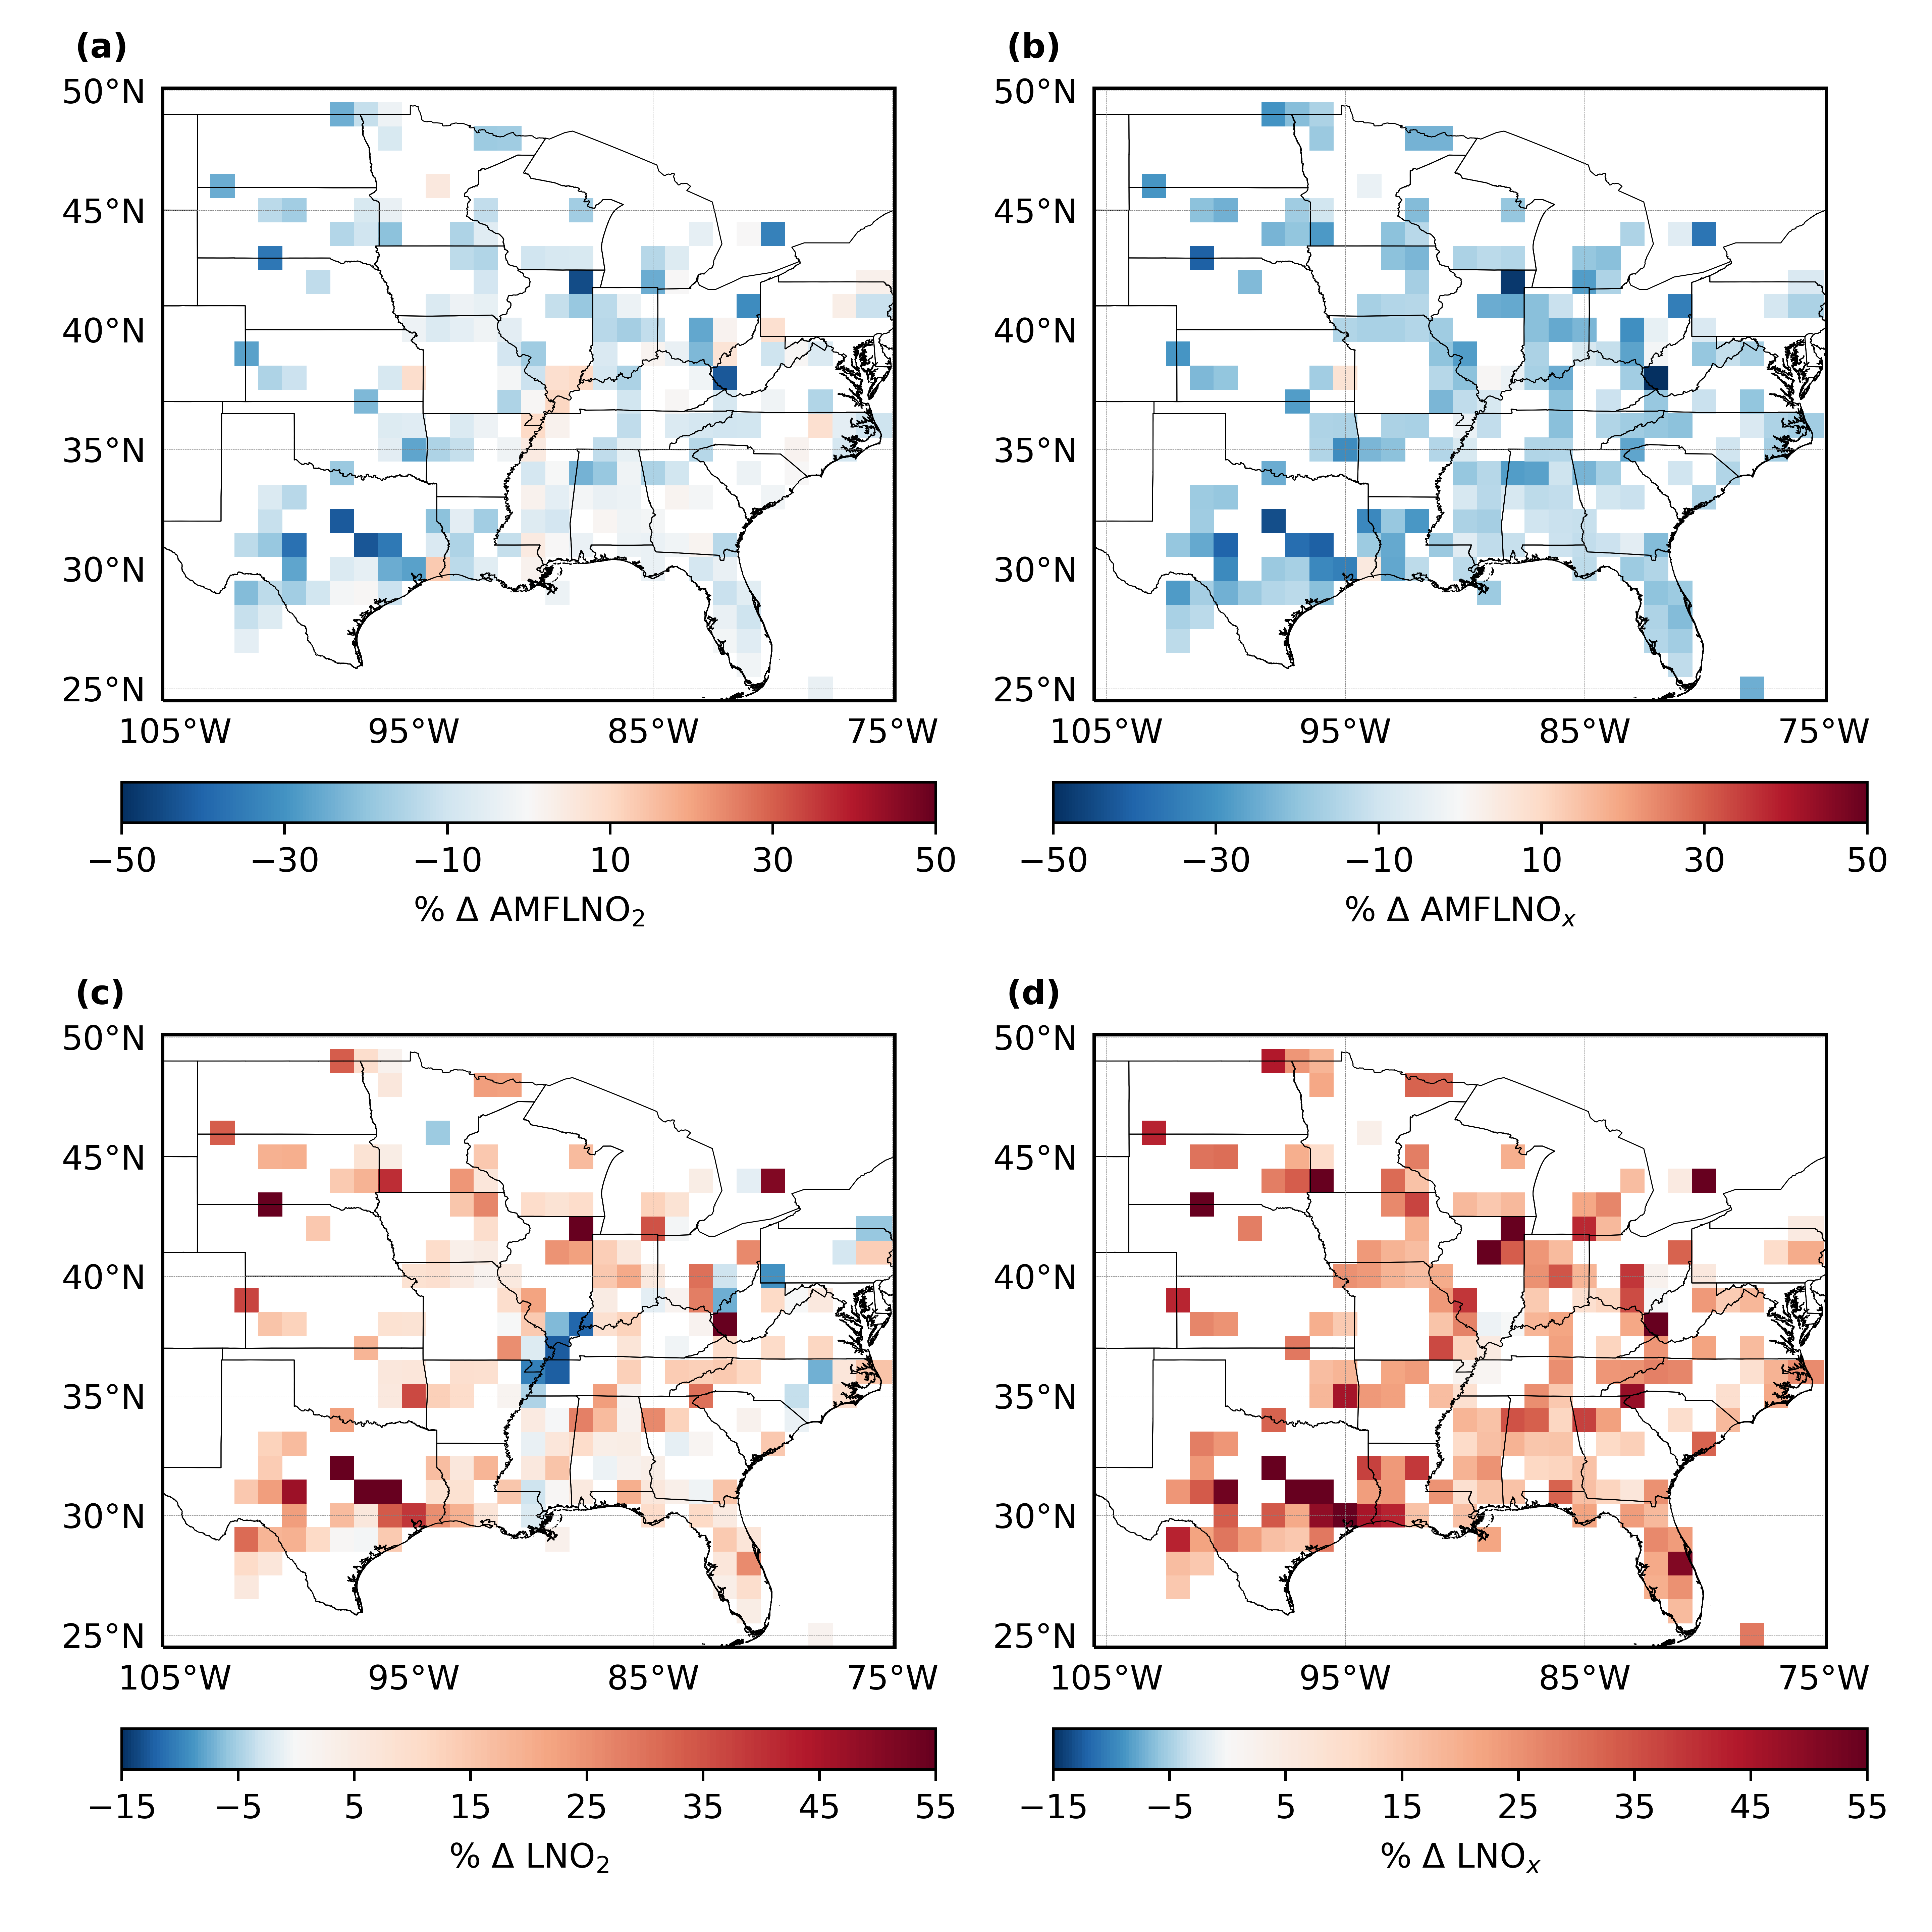
\includegraphics[width=0.95\textwidth]{./figures/us_simulation_diff.png}
\caption{2014年5--8月在CRF $\geq$ 90\% 条件下,
(a)AMF$_{\textrm{LNO$_{\ch{2}}$}}$;(b)AMF$_{\textrm{LNO$_{\ch{x}}$}}$;
(c)LNO$_\textrm{2}$ 和 (d) LNO$_\textrm{x}$的平均百分比差异。
该差异为 2$\times$500 mol NO每闪电 和 1$\times$200 mol NO每闪电所得结果之差。\\
Figure \ref{fig:us_simulation_diff}. Average percent differences in (a) AMF$_{\textrm{LNO$_{\ch{2}}$}}$, (b) AMF$_{\textrm{LNO$_{\ch{x}}$}}$, (c) LNO$_\textrm{2}$ and (d) LNO$_\textrm{x}$ with CRF $\geq$ 90\% over MJJA 2014.
Differences are generated by 2$\times$500 mol NO flash$^{-1}$ and 1$\times$200 mol NO flash$^{-1}$.}
\label{fig:us_simulation_diff}
\end{figure}


图\ref{fig:us_lno2_profile}显示了两个特定区域的平均 LNO 和 LNO$_{\ch{2}}$ 曲线的比较,
其中 2$\times$500 mol NO 每闪电设置分别导致两区域更低和更高的 LNO$_{\ch{2}}$产率。
第一个所选区域(36--37$^{\circ}$ N,89--90$^{\circ}$ W,图\ref{fig:us_lno2_profile}a)是 LNO$_{\ch{2}}$ 负百分比变化最小的区域(图\ref{fig:us_simulation_diff}c),
第二个所选区域(31--32$^{\circ}$ N,97--98$^{\circ}$ W,图\ref{fig:us_lno2_profile}b)是LNO$_{\ch{2}}$ 正百分比变化最大的区域(图\ref{fig:us_simulation_diff}c)。
尽管两个区域的平均 LNO 和 LNO$_{\ch{2}}$廓线的相对分布相似,但量级相差10 倍。
这意味着 WRF-Chem中闪电参数化的表现具有区域性,并且对流层上层可能会出现不切实际的廓线。
虽然这种敏感性分析在某些地区是错误的,但它可得到由于 LNO 和 LNO$_{\ch{2}}$ 廓线而影响NO$_{\ch{2}}$的上限。
正如\citet{Laughner.2017}中所讨论的,在多云条件下散射权重是均匀的,并且由于高反照率,NO$_{\ch{2}}$ 的灵敏度在不同高度上几乎是恒定的。
但是,本研究应仔细考虑对流层上层LNO$_{\ch{2}}$ 的相对分布。
如果云层上方的 LNO$_{\ch{2}}$ ∕ NO$_{\ch{2}}$ 足够大(图\ref{fig:us_lno2_profile}a),
AMF$_{\ch{LNO2}}$ 很大程度上取决于 LNO$_{\ch{2}}$Vis 与 LNO$_{\ch{2}}$ 的比值,
即与相对分布有关。
当不满足高 LNO$_{\ch{2}}$ ∕ NO$_{\ch{2}}$ 的条件时,相对分布和比例都很重要(图\ref{fig:us_lno2_profile}b)。


\begin{figure}[H]
\centering
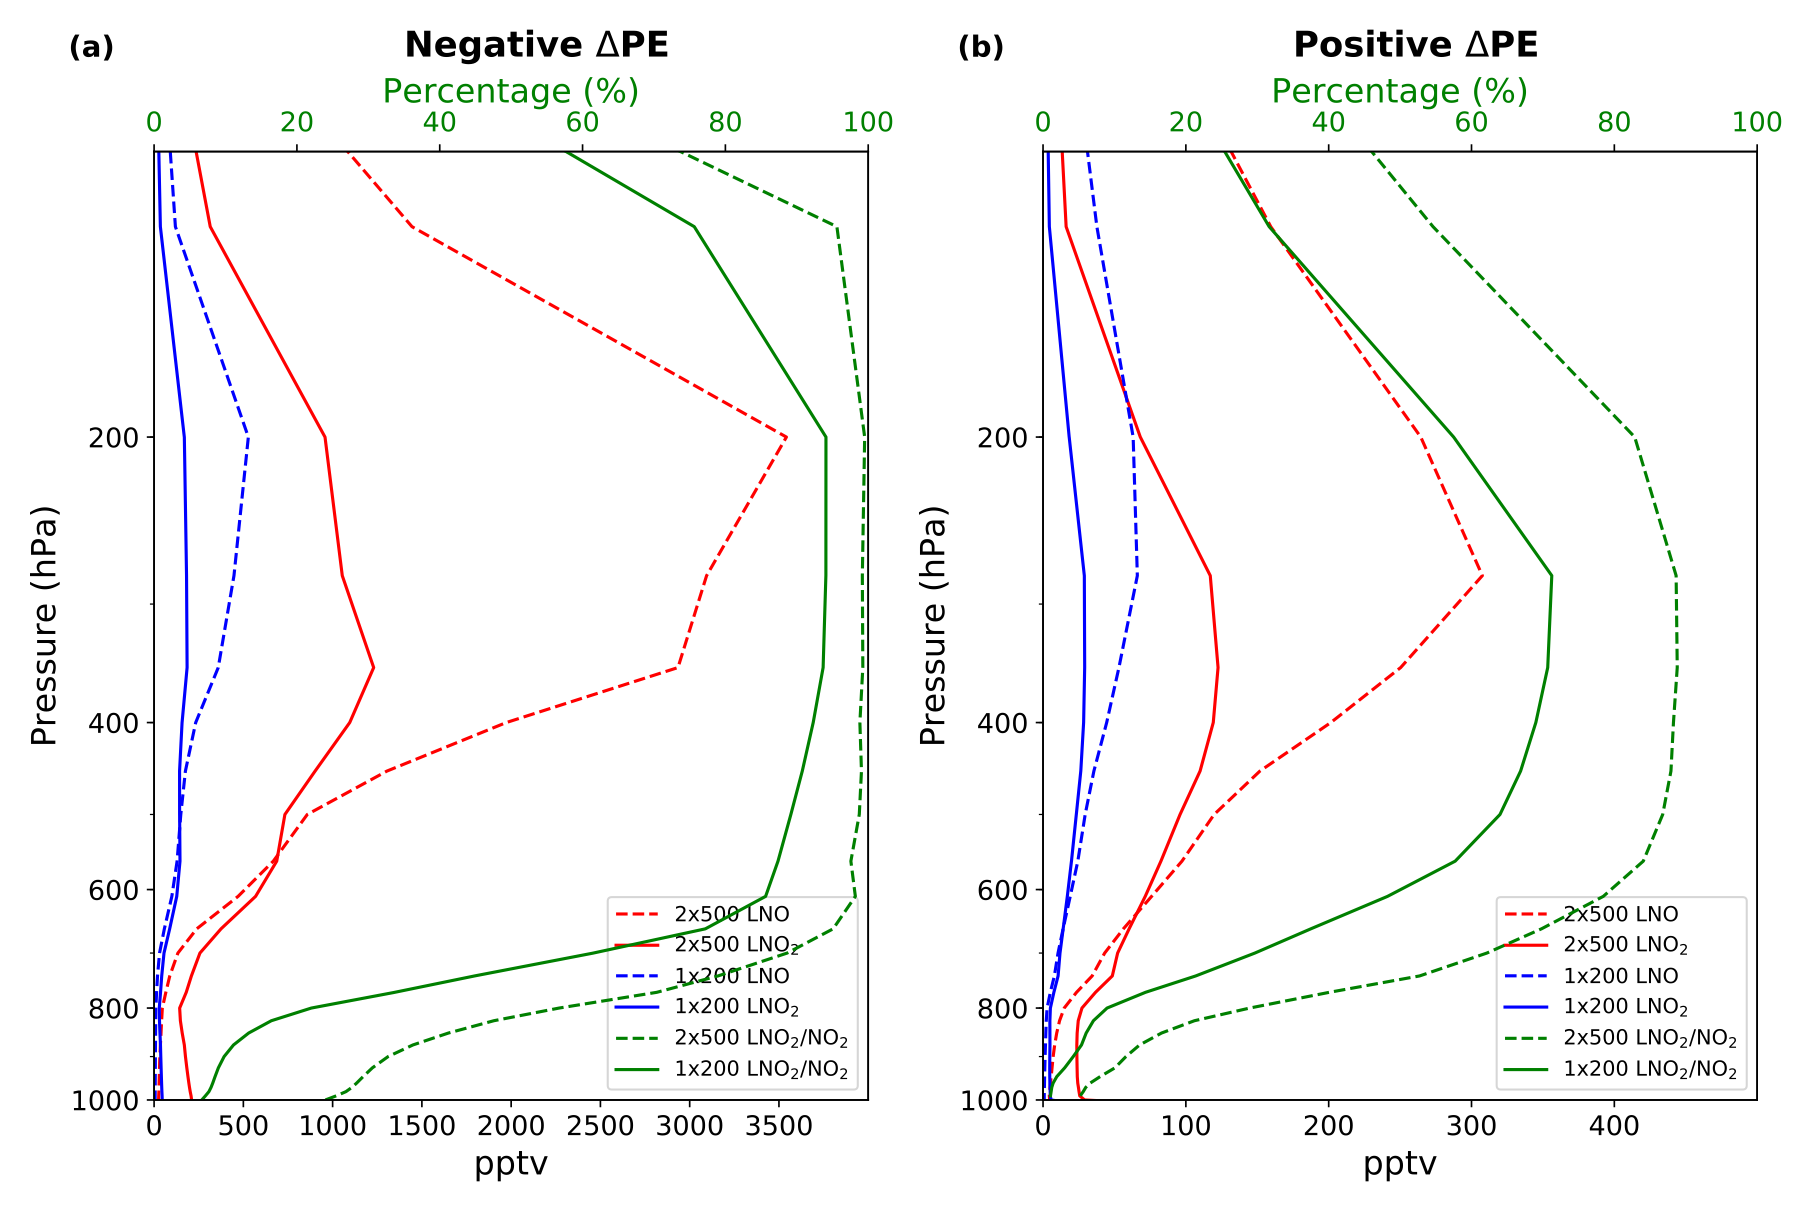
\includegraphics[width=0.95\textwidth]{./figures/us_lno2_profile.png}
\caption{当LNO 设置从 1$\times$200 mol NO每闪电 更改为 2$\times$500 mol NO每闪电 时,
(a)包含 LNO$_{\ch{2}}$ 的最小负百分比变化的区域和(b)包含最大正百分比变化的区域中LNO 和 LNO$_{\ch{2}}$ 的平均廓线廓线。
使用 1$\times$200(2$\times$500)mol NO每闪电的曲线以蓝色(红色)线显示。
绿色实线(虚线)是 在1$\times$200(2$\times$500)mol NO每闪电设置下LNO$_{\ch{2}}$ 与 NO$_{\ch{2}}$ 的平均比例。\\
Figure \ref{fig:us_lno2_profile}. LNO and LNO$_{\ch{2}}$ profiles with different LNO settings at (a) the region containing the minimal negative percent change in LNO$_{\ch{2}}$ and (b) the region containing the largest positive percent change in LNO$_{\ch{2}}$ when the LNO setting is changed from 1$\times$200 mol NO flash$^{-1}$ to 2$\times$500 mol NO flash$^{-1}$, averaged over MJJA 2014.
The profiles using 1$\times$200 (2$\times$500) mol NO flash$^{-1}$ are shown in blue (red) lines.
Solid (dashed) green lines are the mean ratio of LNO$_{\ch{2}}$ to NO$_{\ch{2}}$ with 1$\times$200 (2$\times$500) mol NO flash$^{-1}$.}
\label{fig:us_lno2_profile}
\end{figure}

为了说明这一点,本研究使用了不同的LNO产率设置来对LNO$_{\ch{2}}$、LNO$_{\ch{2}}$Vis、LNO$_{\ch{2}}$Clean 和 NO$_{\ch{2}}$Vis进行敏感性试验(图\ref{fig:us_lno2_profile})。
其中CRF 的阈值设置为 100\% 以简化等式。
总体上来说,LNO$_{\ch{2}}$Clean 和 NO$_{\ch{2}}$Vis 的差异小于 LNO$_{\ch{2}}$ 和 LNO$_{\ch{2}}$Vis 的差异。
通过比较方程中的分子和分母,可得知为何不同的LNO排放设置产生的影响在图\ref{fig:us_lno2_profile}c和d中较小。
对于 LNO$_{\ch{2}}$Clean 和 NO$_{\ch{2}}$Vis,当更多(更少)LNO$_{\ch{2}}$ 或 NO$_{\ch{2}}$ 存在时,S$_{\ch{NO2}}$ 和 V$_{\ch{NO2}}$ 都会增加(减少)。
图\ref{fig:us_lno2_profile}a和b的区别是分母,分别为总对流层 LNO$_{\ch{2}}$ 垂直柱浓度和可见 LNO$_{\ch{2}}$ 垂直柱浓度,
因此图\ref{fig:us_lno2_profile}a中的负值是由云下的 LNO$_{\ch{2}}$ 部分引起的。
该误差可导致LNO$_{\ch{2}}$ 和 LNO$_{\ch{x}}$产率的不确定性,本研究保守估计分别为 $\pm$13\% 和 $\pm$25\%。
最终LNO$_{\ch{2}}$ 和 LNO$_{\ch{x}}$产率的不确定性是根据\citet{Pickering.2016,Allen.2019,Bucsela.2019,Lapierre.2020}的方法得到,即通过依次扰动每个参数来重新计算LNO$_{\ch{2}}$ 和 LNO$_{\ch{x}}$,从而得到不确定性(表\ref{table:us_uncertainty})。


本研究使用与 NASA 标准产品一致的 GEOS-5 月平均对流层顶气压,而不是可变的 WRF 对流层顶高度来评估由 BEHR 对流层顶压造成的不确定性。
\citet{Acarreta.2004}等人将云压偏差用云压和云分数的函数表示,依此岑研究得到计算的LNO$_{\ch{2}}$产率不确定性为 32\%,
LNO$_{\ch{x}}$产率不确定性为 34\%,这是产率估算中不确定性的最大来源。
接着,由于GLOBE地形高度数据的分辨率远高于OMI像素,在BEHR算法中采用假设的固定比例高度,
因此\citet{Laughner.2019a}将 WRF 平均地表气压与 GLOBE 地表气压进行了比较,得出最大偏差为 1.5\%。
基于最大偏差,本研究改变了地表气压并限制其小于 1020 hPa,得到的不确定性可忽略不计。

云辐射分数的误差可由云分数得到
\begin{equation}
\sigma = 0.05 \times \left.\frac{\partial{f_r}}{\partial{f_g}}\right|_{f_{g,pix}}
\end{equation}
其中 $f_r$ 是云辐射度分数,$f_g$ 是云分数,$f_{g,pix}$ 是特定像素的云分数。
对于 LNO$_{\ch{2}}$ 和 LNO$_{\ch{x}}$产率,云分数的误差转换为 2\% 的云辐射分数误差。

500m MODIS 反照率产品的精度通常在站点反照率观测值的 5\% 以内,而那些低质量的异常值主要在观测数据的 10\% 以内\citep{Schaaf.2011}。
由于本研究直接使用双向反射率分布函数(BRDF)数据,而不包含辐射传输模型,
因此将 14\% 的朗伯等效反射率误差和 10\% 的不确定性结合起来得到 17\% 的扰动\citep{Laughner.2019a},重新计算结果显示该扰动对于估算的影响也可忽略。

与 NASA 标准产品 v2 相比,\citet{Krotkov.2017}证明V$_\textrm{strat}$中的误差为 10$^{14}$ cm$^{-2}$。
在污染区域该误差可能略大于此值,而在最清洁区域的误差通常要小得多\citep{Bucsela.2013}。
依据\citet{Allen.2019},本研究估计V$_\textrm{strat}$分量的不确定性和斜柱误差分别为 10\% 和 5\%。

基于美国大陆上相对于 LIS 的探测效率,ENTLN 探测效率的不确定性对于云闪为 $\pm$ 16\%,
由于地闪 在美国大陆具有高探测效率,不确定性估计为 $\pm$ 5\% \citep{Lapierre.2020},由此产生的估算不确定度为15\%。
此外,本研究使用 2.4 h 的时间窗口中的ENTLN闪电和闪击来分析 NO$_{\ch{2}}$ 和 LNO$_{\ch{x}}$ 的产率。
由于从 ERA5 再分析得出的时间窗口不能代表可变风速,因此进行了敏感性试验。
使用 2 和 4 h 的时间窗口得出闪电产量的不确定性为 10\%,闪击产量的不确定性为 8\%。
此外,对流层上层NO$_{\ch{x}}$ 的寿命范围为 2--12 h,具体取决于对流位置、过氧硝酸甲酯、烷基以及多功能硝酸盐\citep{Nault.2017}。
本研究将方程式中的6 h用 2 h和 12 h 代替,从而得到由于寿命导致的不确定性为 24\%,
这与 LNO$_{\ch{x}}$ 类型的闪电参数化引起的不确定性(25\%)相当。

最近的研究表明,模拟的 NO ∕ NO$_{\ch{2}}$比例与 SEAC4RS 飞机观测的数据不同\citep{Travis.2016,Silvern.2018}。
\citet{Silvern.2018}将此归因于对 NO$_{\ch{2}}$ 测量的正干扰或低温 NO--NO$_{\ch{2}}$--O$_{\ch{3}}$ 光化学反应速率的误差。
考虑到可能的 NO$_{\ch{2}}$ 测量正干扰\citep{Allen.2019,Bucsela.2019},
本研究为该误差分配 20\% 偏差和 $\pm$ 15\% 不确定性,并估计产率的不确定性为 15\%。

此外LNO$_{\ch{x}}$产率的估算还取决于对流层背景NO$_{\ch{2}}$浓度。
在本研究中影响该因素的主要因素是排放清单和传输的 NO$_{\ch{2}}$。
对于排放清单,不确定性的来源是假设条件、计算方法、输入数据和计算误差。
因此与 NO$_{\ch{2}}$ 相关的不同物种或污染物的不确定性是不同的。
对于模拟的对流传输,\citet{Li.2018}将云解析模拟与基于对流参数化的模拟进行了比较,并指出对流输送在参数化中较弱。
但是,比例条件(LNO$_{\ch{2}}$Vis/NO$_{\ch{2}}$Vis $\geq$ 50\%)应该减少了这两种不确定性,
本研究假设背景NO$_{\ch{2}}$浓度导致的不确定性为 10\%,小于 \citet{Allen.2019}和\citet{Bucsela.2019}等研究中使用的 20\%。

净不确定性为表\ref{table:us_uncertainty}中所有单个不确定性平方和的平方根。
LNO$_{\ch{2}}$ 类型和 LNO$_{\ch{x}}$ 类型的净不确定性分别为 48\% 和 56\%。
基于线性回归和求和法的平均结果为32 mol NO$_{\ch{2}}$每闪电、90 mol NO$_{\ch{x}}$每闪电、6 mol NO$_{\ch{2}}$每闪击 和 17 mol NO$_{\ch{x}}$每闪击。
将相应的不确定性应用于这些平均值,本研究得出32 $\pm$ 15 mol NO$_{\ch{2}}$每闪电、90 $\pm$ 50 mol NO$_{\ch{x}}$每闪电、
6 $\pm$ 3 mol NO$_{\ch{2}}$每闪击 和17 $\pm$ 10 mol NO$_{\ch{x}}$每闪击。
这在当前文献估计(33--500 mol NO$_{\ch{x}}$每闪电)的范围内\citep{Schumann.2007,Beirle.2010,Bucsela.2010}。
最近\citet{Bucsela.2010}研究中估算的LNO$_{\ch{x}}$产率为 100--250 mol NO$_{\ch{x}}$每闪电,高于但与本研究结果相重叠。
\citet{Pickering.2016}估算的墨西哥湾LNO$_{\ch{x}}$产率为 80 $\pm$ 45 mol NO$_{\ch{x}}$每闪电,比本研究中美国大陆的结果低50\%。
因为墨西哥湾上空有许多缺失数据,因此两个研究实际上是不同地区之间的比较。
如果\citet{Pickering.2016}的方法未对背景NO$_{\ch{2}}$进行校正,得出的 LNO$_{\ch{x}}$产率在清洁区域或云上LNO$_{\ch{2}}$浓度高的区域与本研究相似,但在污染区域高估18\%以上。
对于基于闪击的结果,\citet{Lapierre.2020}得到的LNO$_{\ch{2}}$产率较低,为1.6 $\pm$ 0.1 mol NO$_{\ch{2}}$每闪击。
该差异是由不同版本的 BEHR 算法和其他设置引起的,由于本研究的方法将云下LNO$_{\ch{2}}$考虑进总的LNO$_{\ch{2}}$,所以得到的LNO$_{\ch{2}}$产量可能会更大,尤其是对于高的云层。

\begin{table}[H]
\centering
\caption{估算LNO$_{\ch{2}}$和LNO$_{\ch{x}}$产率的不确定性\\ Table \ref{table:us_uncertainty}. Uncertainties for the estimation of LNO$_{\ch{2}}$ and LNO$_{\ch{x}}$ production efficiencies (PE).}
\scriptsize
\begin{tabular}{llllll}
\thickline
来源 & 扰动 & NO$_{\ch{2}}$每闪电$^e$ & NO$_{\ch{x}}$每闪电$^e$ & NO$_{\ch{2}}$每闪击$^e$ & NO$_{\ch{x}}$每闪击$^e$ \\
\thickline
BEHR对流层顶高度$^a$                    & NASA产品                              & 6   & 4   & 6   & 4 \\
云辐射分数$^a$                          & $\pm$ 5\%                            & 2   & 2   & 2   & 2 \\
云压$^b$                               & 变化的                                & 32  & 34  & 32  & 34 \\
地表气压$^a$                            & $\pm$ 1.5\%                          & 0   & 0   & 0   & 0 \\
地表反照率$^a$                          & $\pm$ 17\%                           & 0   & 0   & 0   & 0 \\
LNO$_{\ch{2}}$廓线$^a$               & 2$\times$500 mol NO每闪电             & 13  & 25  & 13  & 25 \\
廓线位置$^a$                            & 拟蒙特卡罗法                           & 0   & 1   & 0   & 1 \\
闪电探测效率$^c$                        & 云闪: $\pm$ 16\%, 地闪: $\pm$ 5\%        & 15  & 15  & 15  & 15 \\
时间窗口%
$^c$                                  & 2 -- 4 hours                         & 10  & 10  & 8   & 8 \\
LNO$_{\ch{x}}$寿命%
$^c$                                  & 2 -- 12 hours                        & 24  & 24  & 24  & 24 \\
V$_{strat}$%
$^d$                                  & -                                    & 10  & 10  & 10  & 10 \\
斜柱浓度的系统误差$^d$                   & -                                    & 5   & 5   & 5   & 5 \\
对流层背景浓度$^d$           & -                                    & 10  & 10  & 10  & 10  \\
NO/NO$_{\ch{2}}$%
$^d$                                  & 20\% $\pm$ 15\%                      & 0   & 15  & 0   & 15 \\
净                                   & -                                    & 49  & 56  & 48  & 56 \\
\thickline
\end{tabular}
\begin{tablenotes}
\linespread{1}\footnotesize
\item PE$_{\ch{不确定性}}$ = (误差$_{\ch{高扰动值}}$ - 误差$_{\ch{低扰动值}}$)/2,
其中 误差$_{\ch{\* 扰动值}}$ = (PE$_{\ch{\* 扰动值}}$ - PE$_{\ch{原始值}}$)/PE$_{\ch{原始值}}$。
\item PE$_{\ch{uncertainty}}$ = (Error$_{\ch{rising\ perturbed\ value}}$ - Error$_{\ch{lowering\ perturbed\ value}}$)/2
where Error$_{\ch{\* perturbed value}}$ = (PE$_{\ch{\* perturbed\ value}}$ - PE$_{\ch{original\ value}}$)/PE$_{\ch{original\ value}}$.
\item $^a$ \citet{Laughner.2019a}, $^b$ \citet{Acarreta.2004}, $^c$ \citet{Lapierre.2020}, $^d$ \citet{Allen.2019} and\ \citet{Bucsela.2019}, $^e$ Uncertainty (\%)
\end{tablenotes}
\label{table:us_uncertainty}
\end{table}

\section{本章小结}

本章基于卫星遥感NO$_{\ch{2}}$柱浓度,开发了不同污染背景下LNO$_{\ch{2}}$的
反演方法,得到了不同污染程度地区的LNO$_{\ch{x}}$产率,并与其他NO$_{\ch{x}}$排放源进行了对比。主要结论如下:

\begin{enumerate}[label=(\arabic*), labelindent=\parindent, nosep, leftmargin=0pt, widest=0, itemindent=*, topsep=0pt, partopsep=0pt, parsep=0pt]

\item 针对污染地区的深对流,本研究利用WRF-Chem的高分辨率模拟结果,
定义了LNO$_{\ch{2}}$和LNO$_{\ch{x}}$的大气质量因子(AMF),
从而得到包含了云下LNO$_{\ch{2}}$和LNO$_{\ch{x}}$的柱浓度。
本研究设置了云辐射分数阈值($\geq$70\%或90\%)、
地基探测的闪电阈值(OMI过境前2.4小时内 1$^{\circ}$ $\times$ 1$^{\circ}$网格中闪电至少2400次或闪击至少8160次)、
模拟的闪电数$\geq$1000 和云上LNO$_{\ch{2}}$占比$\geq$50\%的条件,以确保WRF-Chem 成功模拟出对流并且LNO$_{\ch{2}}$能够被OMI检测。
由于新定义的AMF考虑了对流层的背景污染,因此该方法较前人方法的改进之处在于可以同时适用于清洁和污染区域。

\item 与\citet{Lapierre.2020}相比,本研究的方法考虑了云下LNO$_{\ch{2}}$,
因此在高云的条件下得到的LNO$_{\ch{2}}$ 产量将更大。
此外,若\citet{Pickering.2016}所使用的方法没有对背景NO$_{\ch{2}}$进行校正,其得到的LNO$_{\ch{2}}$产率与本研究在清洁区域或云上方LNO$_{\ch{2}}$ 浓度高的区域相似,但在污染区域可能引起超过18\%的高估。

\item 2014年5--8月的分析结果表明,美国大陆夏季的 LNO$_{\ch{2}}$ 和 LNO$_{\ch{x}}$平均产率为
32 $\pm$ 15 mol NO$_{\ch{2}}$每闪电、90 $\pm$ 50 mol NO$_{\ch{x}}$每闪电、6 $\pm$ 3 mol NO$_{\ch{2}}$每闪击,以及17 $\pm$ 10 mol NO$_{\ch{x}}$每闪击。
然而,由于现阶段其他地区(如中国和印度)NO$_{\ch{2}}$ 污染比美国大陆严重,
在估算LNO$_{\ch{x}}$时需要详细考虑背景污染。
此外区域和全球模式还需开发更为完善的闪电参数化,以提高局地和全球范围内LNO$_{\ch{x}}$排放估算的准确性。

\end{enumerate}
